\documentclass[12pt,a4paper,notitlepage]{article} 

% Adjust margins and spacing
\usepackage{geometry}
% Page margins
\geometry{margin=2.5cm,top=3.5cm,bottom=3cm}
% Line spacing
\renewcommand{\baselinestretch}{1.5}

% Document is in english
\usepackage[english]{babel}

% For splitting equations into several lines
\usepackage{amsmath}

% For using subfigures
\usepackage{subcaption}

% For
% highlighting columns in a table
% using links without bordered box colors
% storing as archived pdf
\usepackage{graphicx}
\usepackage[table]{xcolor}
\usepackage[colorlinks=true,
            allcolors=blue,
            pdfa]{hyperref}

% For using appendic
\usepackage[page,toc,titletoc,title]{appendix}

% For using Natural Sciences-references
\usepackage{cleveref}
\usepackage[round]{natbib}
\bibliographystyle{apalike}

% For rotating the table
\usepackage{rotating}

% For archived pdf
\usepackage{pdfpages}

% Using multirows in tables
\usepackage{multirow}

% Adjusting box propertines in table
\usepackage{adjustbox}

% For rotating the column headers in table
\usepackage{array}
\usepackage{hyphenat}

% Archived pdf
\usepackage[a-2b,mathxmp]{pdfx}[2018/12/22]

% Using specific styles for (table, figure etc.) captions
\usepackage[font={small,it}]{caption}

% Drawing dashed lines in tables
\usepackage{arydshln}

% Using specific checkmarks in tables when indicating whether certain controls are included or not
\usepackage{pifont}

% New command for rotating columd header in table
\newcolumntype{R}[2]{%
    >{\adjustbox{angle=#1,lap=\width-(#2)}\bgroup}%
    l%
    <{\egroup}%
}
\newcommand*\rot{\multicolumn{1}{R{45}{1em}}}

% For highlighting the main specification with gray
\newcolumntype{a}{%
    >{\columncolor[gray]{.9}[0pt]}%
    c%
}

% For adjusting box size
\usepackage[graphicx]{realboxes}
\newcommand\Tstrut{\rule{0pt}{2.6ex}}
\newcommand\Bstrut{\rule[-0.9ex]{0pt}{0pt}}

% For using superscripts in texts. Like 2nd, 3rd, 10th...
\newcommand{\ts}{\textsuperscript}

% For control status checkmarks
\definecolor{darkgreen}{rgb}{0.0, 0.29, 0.29}
\definecolor{darkred}{rgb}{0.34, 0.01, 0.1}
\newcommand{\cmark}{\color{darkgreen}{\ding{51}}}%
\newcommand{\xmark}{\color{darkred}{\ding{55}}}%

% Image path
\graphicspath{{images/}}

\title{The Effect of COVID-19 on Health Outcomes in Developing Countries – an Empirical Study from India}
\author{Tuomas Tölli}
\makeatletter
\let\ititle\@title
\let\iauthor\@author
\makeatother

\begin{document}

\pagenumbering{gobble}

% Remember that these needs to be in PDFA/2-format already before inclusing! Otherwise it's not possible for final document either
% Cover page
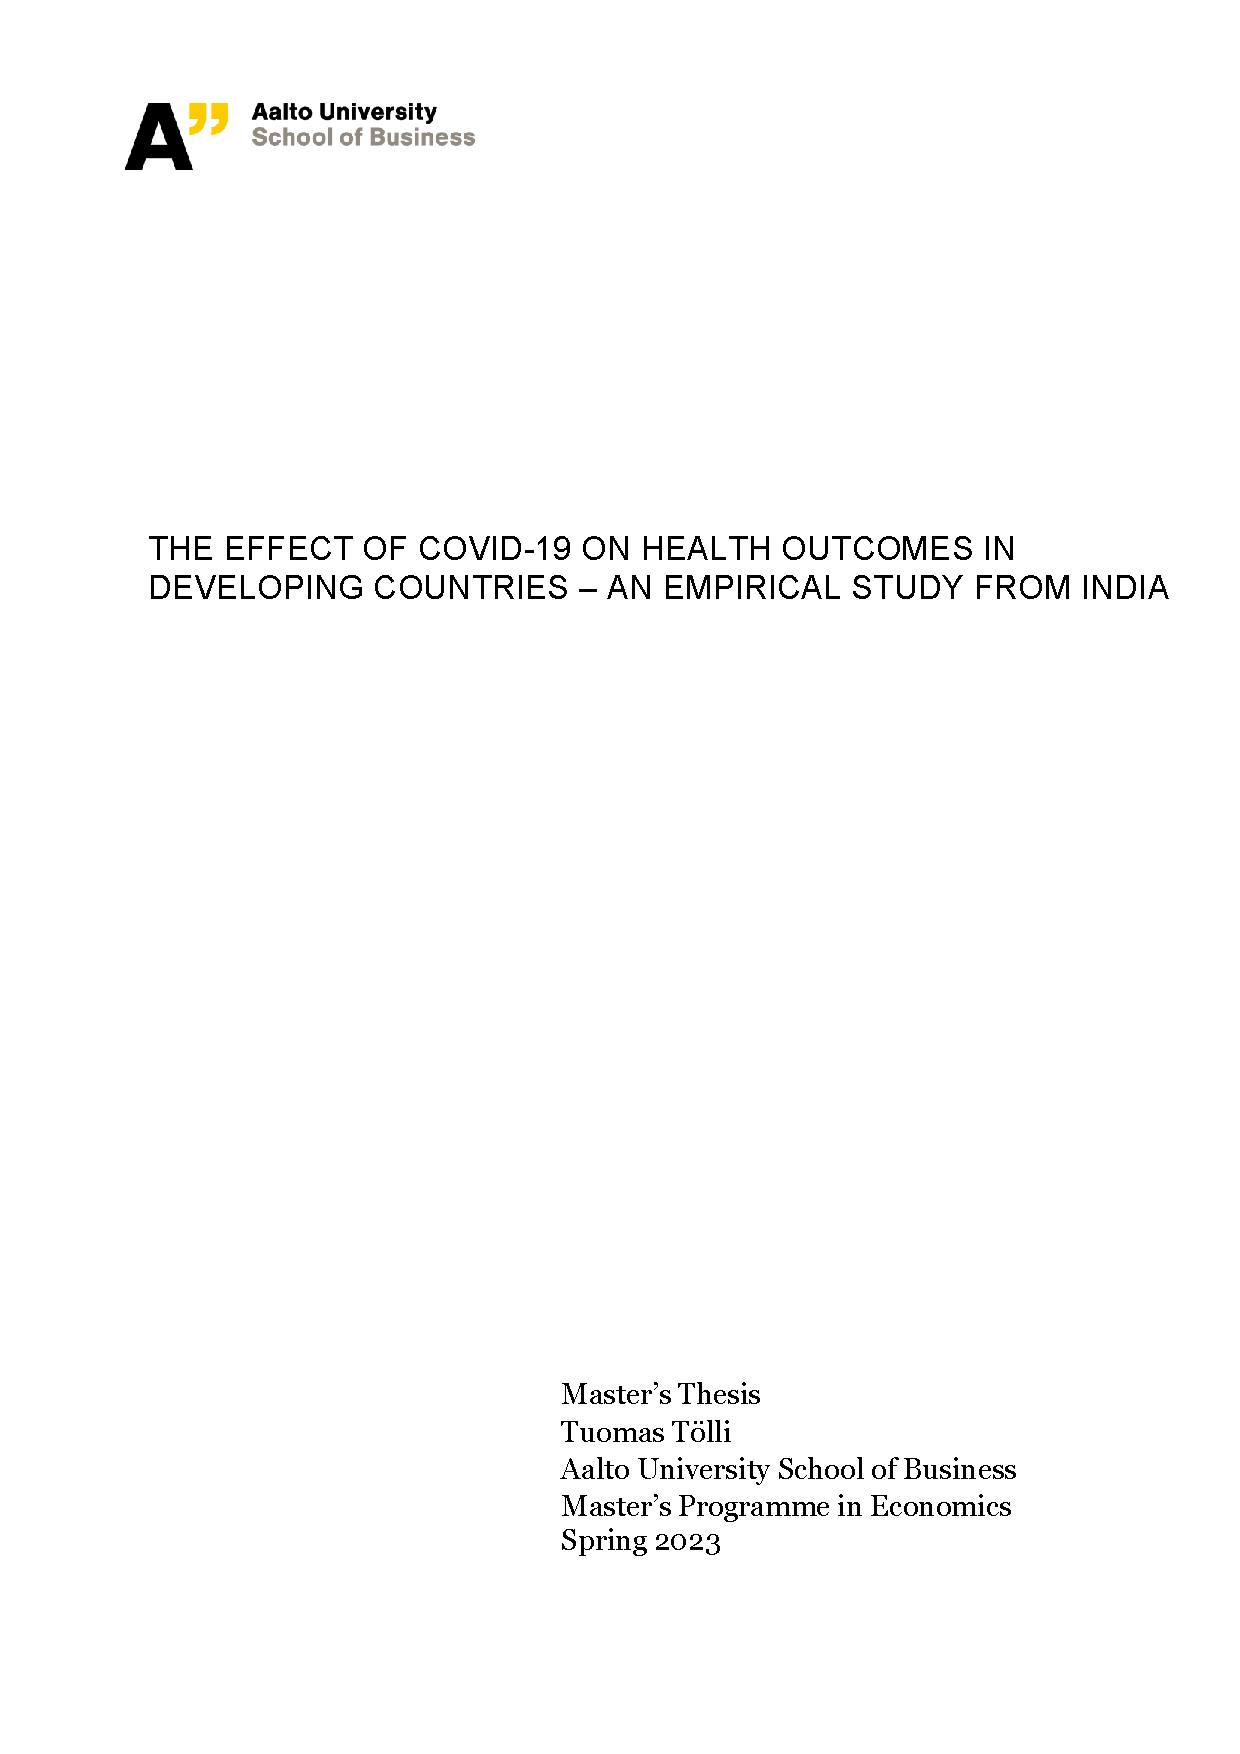
\includepdf[pagecommand={\thispagestyle{empty}},pages=-]{cover/cover.pdf}

% English abstract
%The detailed effects of the COVID-19 pandemic on e.g., global poverty is not yet fully known. How-ever, it seems obvious that there have been effects, and that the strength of the effects may also vary depending on the countries’ demographic structure and level of economic development. This work examines health, which is not only significantly related to poverty, but also an important background factor for economic growth and development. The research question is whether there have been changes on health outcomes in developing countries during the COVID-19 pandemic. The focus is on the indirect effects operating through economic channels, which are examined separately from the direct health effects of infected people. The thesis is carried out with the help of fifth Demographic and Health Survey (DHS) of India. In addition, the work makes use of the full lockdowns that unexpectedly and unpredictably stopped data collection for six months in March 2020. The thesis briefly reviews the literature related to health and economic development. Thereafter, 14 different health outcomes are selected for more detailed research. These outcomes that have been shown to be associated with later economic development are related to immunization levels, nutrition, exposure to domestic violence, alcohol usage and smoking level. In the empirical part, probit and OLS models are built to investigate potential changes in selected health outcomes during the first wave of COVID-19 pandemic. In addition to the time of the inter-view, household wealth is also used as a variable of interest. Data balance and model robustness are addressed separately. In addition, a detailed analysis of vaccination- and nutrition outcomes of children is performed, using the guidelines and indicators set by WHO. To account for possible long-term trends, the results are compared to figures from previous DHS surveys. Finally, the Oxford COVID-19 Government Response Tracker (OxCGRT) dataset is used to examine possible differences that may have been due to differences in adopted policy responses by states. The results seem to be twofold. Improving development in immunization coverage in recent years seems to have stalled in India. The long-terms downward trend in the proportion of under-weight children in low-wealth households also seems to have stopped. In addition, nutritional indicators seem to have worsened, especially among breastfed children. On the other hand, the proportion of anaemic children and adults appears to have decreased significantly. In addition, the results related to men’s smoking and alcohol use and women’s experience of domestic violence have improved significantly. The results indicate that the sudden and complete lockdowns imposed by India in March-May 2020 may have indirectly affected health outcomes.
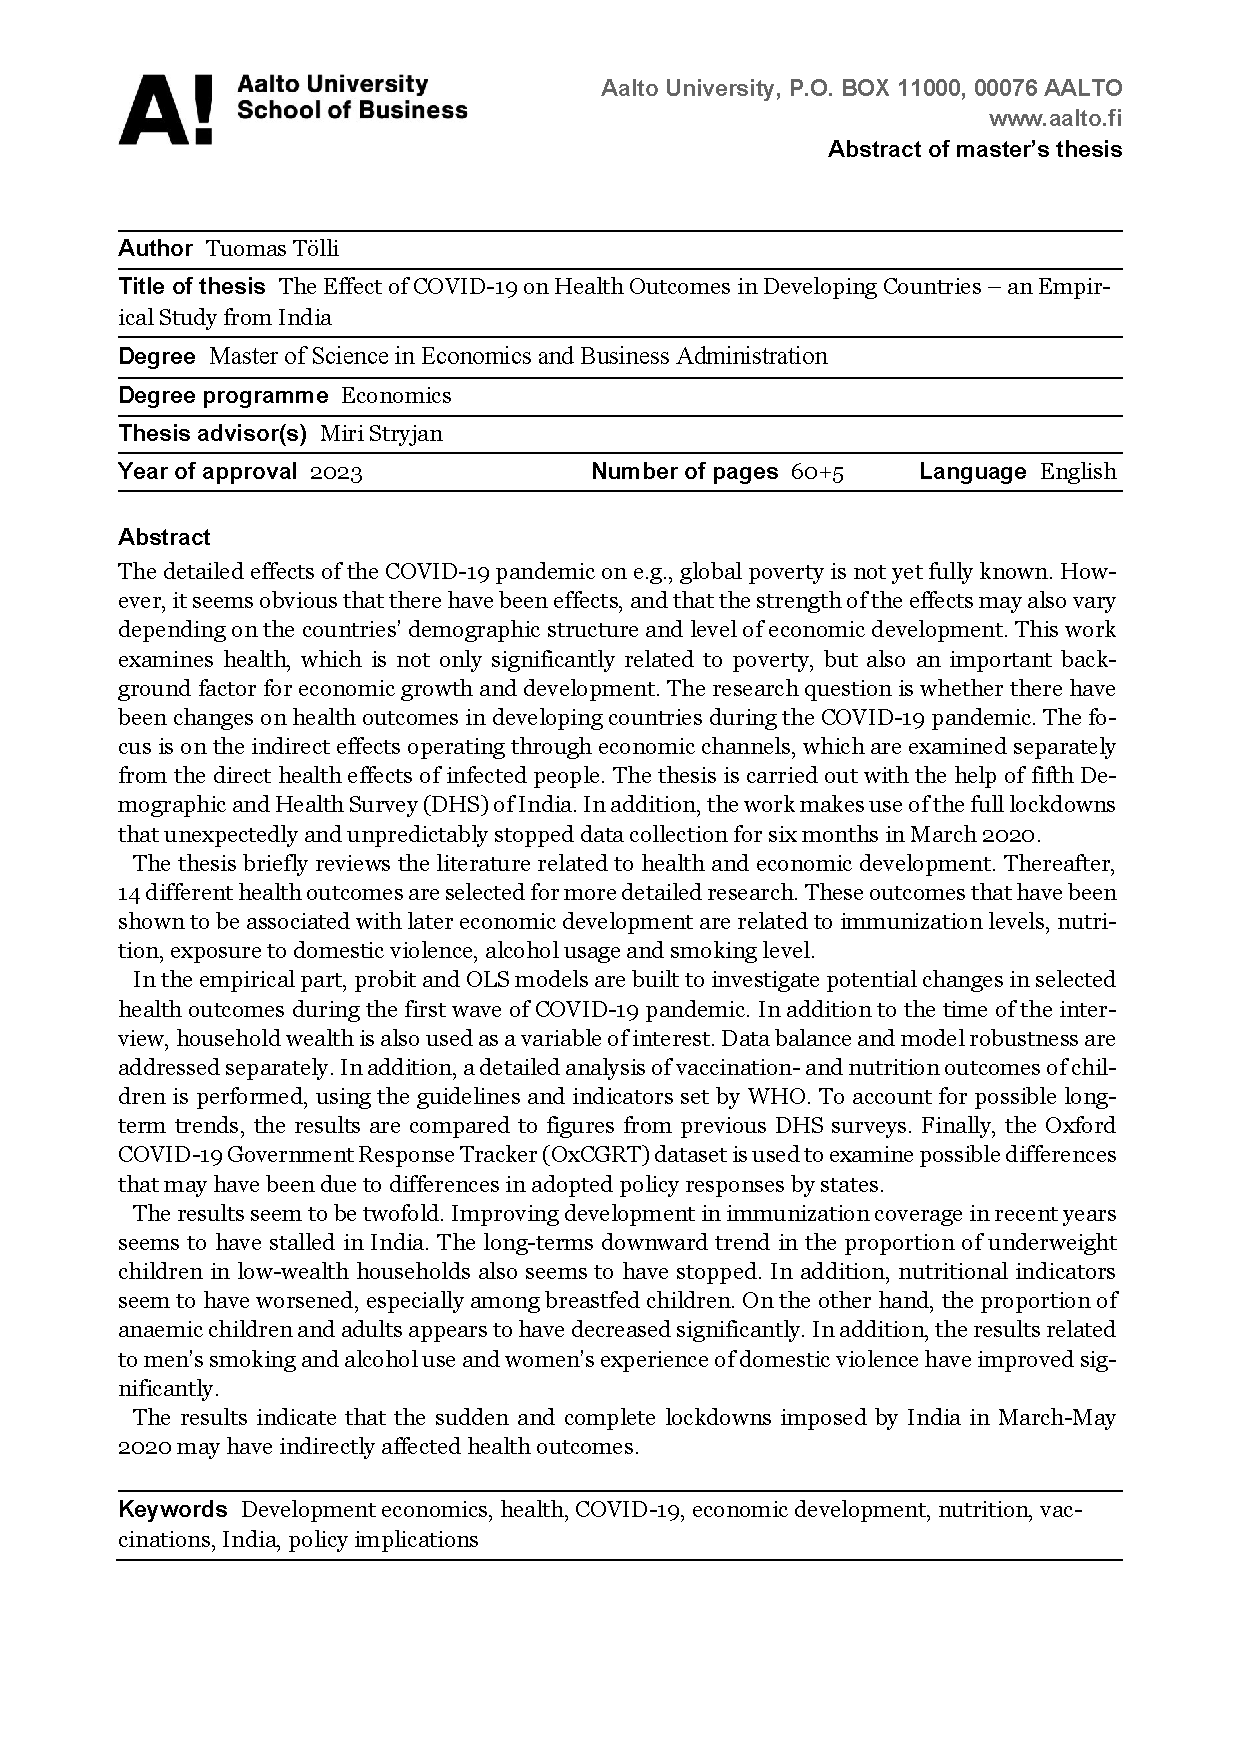
\includepdf[pagecommand={\thispagestyle{empty}},pages=-]{cover/abstractEn.pdf}

% Finnish abstract
%COVID-19-pandemian yksityiskohtaisia vaikutuksia esimerkiksi globaaliin köyhyyteen ei vielä täy-sin tunneta. Näyttää kuitenkin jokseenkin ilmeiseltä, että vaikutuksia on ollut, ja että vaikutusten voimakkuus saattaa vaihdella maiden väestörakenteen ja taloudellisen kehitystason mukaan. Täs-sä työssä tarkastellaan erityisesti terveyttä, joka on paitsi merkittävässä yhteydessä köyhyyteen, myös tärkeä taustatekijä taloudelliselle kasvulle ja kehitykselle. Työn tutkimuskysymyksenä on, onko kehitysmaiden terveystuloksissa tapahtunut muutoksia COVID-19-pandemian aikana. Pai-nopiste on taloudellisten kanavien kautta tapahtuvissa välillisissä vaikutuksissa, joita tarkastel-laan erillään tartunnan saaneiden suorista terveysvaikutuksista. Työ toteutetaan Intian viidennen väestö- ja terveyskyselyaineiston (Demographic and Health Survey) avulla. Työssä hyödynnetään lisäksi Intian hallituksen asettamia voimakkaita sulkutiloja ja -toimenpiteitä, jotka yllättäen ja odottamatta pysäyttivät tiedonkeruun kuudeksi kuukaudeksi maaliskuussa 2020. Työssä tarkastellaan lyhyesti terveyteen ja taloudelliseen kehitykseen liittyvää kirjallisuutta. Tämän jälkeen valitaan 14 erilaista terveysmuuttujaa tarkempaa tutkimusta varten. Muuttujat, joiden on osoitettu olevan yhteydessä myöhempään taloudelliseen kehitykseen, liittyvät immuni-saatioon, ravitsemukseen, tupakoinnin sekä alkoholinkäytön tasoon ja perheväkivallalle altistumi-seen. Empiirisessä osassa rakennetaan probit- ja OLS-mallit, joilla tutkitaan mahdollisia muutoksia COVID-19-pandemian ensimmäisen aallon aikana. Haastatteluajankohdan lisäksi myös kotita-louksien varallisuutta käytetään mielenkiintomuuttujana. Aineiston tasapainoa ja mallin robusti-suutta käsitellään työssä erikseen. Lisäksi työssä tehdään lapsien rokotus- ja ravitsemustuloksiin liittyvä yksityiskohtainen analyysi, käyttäen WHO:n asettamia ohjeistuksia ja indikaattoreita. Mahdollisia pitkän aikavälin muutoksia varten tuloksia suhteutetaan aiempiin DHS-tutkimuksiin. Lopuksi OxGCRT-aineistoa (Oxford COVID-19 Government Response Tracker) käytetään tutki-maan eroja, jotka ovat saattaneet johtua osavaltioiden harjoittamien politiikkatoimien eroavai-suuksista. Tulokset näyttävät olevan kahtalaisia. Viime vuosien positiivinen kehitys rokotuskattavuudessa näyttää pysähtyneen Intiassa. Myös vähävaraisten kotitalouksien alipainoisten lasten osuuden pitkäaikainen laskusuuntaus näyttää pysähtyneen. Lisäksi erityisesti rintaruokittujen lasten kes-kuudessa ravitsemusindikaattorit näyttävät huonontuneen. Toisaalta anemiasta kärsivien lasten ja aikuisten osuus näyttää pienentyneen merkittävästi. Lisäksi miesten tupakointiin ja alkoholin-käyttöön sekä naisten kokemaan perheväkivaltaan liittyvät tulokset ovat parantuneet. Työssä saatujen tulosten mukaan Intian maalis-toukokuussa 2020 asettamat äkilliset ja täydelli-set sulkutoimenpiteet ovat saattaneet vaikuttaa epäsuorasti terveystuloksiin.
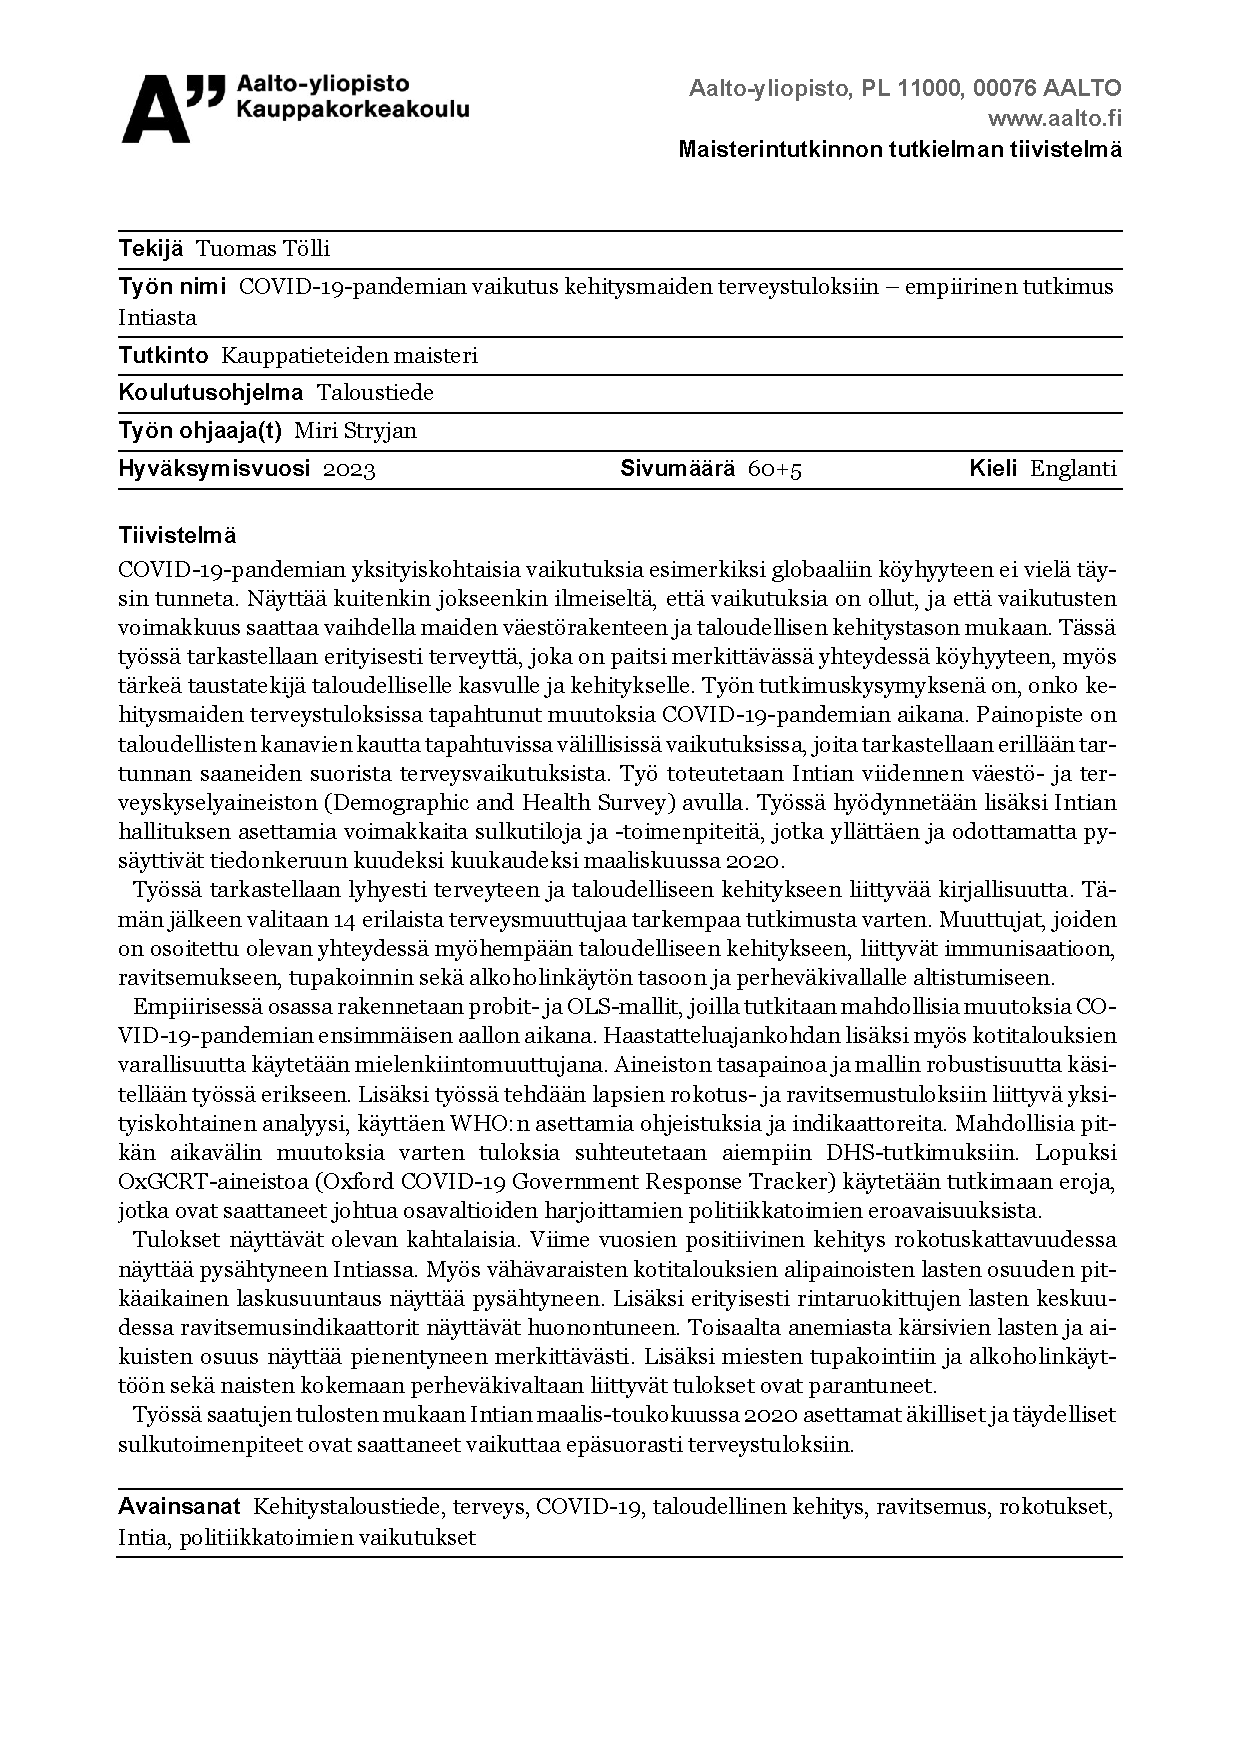
\includepdf[pagecommand={\thispagestyle{empty}},pages=-]{cover/abstractFi.pdf}

{\let\clearpage\relax \tableofcontents} 

\thispagestyle{empty}

\clearpage

\pagenumbering{arabic}

\setcounter{page}{6}

\section{Introduction} \label{sec:introduction}

Measured since the beginning of the pandemic, COVID-19 has caused more than 676 million infections worldwide, of which 6.9 million have ended in death\footnote{\href{https://coronavirus.jhu.edu/map.html}{ COVID-19 Dashboard by the Center for Systems Science and Engineering at Johns Hopkins University}, page accessed 2023-5-12, data collection stopped 2023-3-10}. In addition to the direct impact on those infected, the economic consequences appear to have been considerable. Measuring the effects of COVID-19 on global poverty has not yet been possible, as nationally representative household surveys are not necessarily available from low- and lower middle-income countries. However, according to preliminary estimates, the effect on poverty figures may have been significant. For example, with a combination of real household surveys, high-frequency phone surveys and simulations, \citet{Lakmer:2022} estimated that during 2020 the number of people living in extreme poverty increased by 143 million to the level of five years ago.

Although the COVID-19 pandemic has affected all parts of the world, there are factors that make possible indirect effects more difficult for developing countries to cope with: Government protection programs and other institutional compensations are not as significant as in general in developed countries, because developing countries have less available task resources; a significantly larger part of economic activity takes place in the informal sector, which makes possible state subsidies less efficient; public healthcare infrastructure is also generally weaker; and finally, there are more people with little or no savings that can be used as a buffer in situations like foreclosures that can have longer-term effects. (\citet{Bundervoet:2022,Egger:2021})

There are several studies that show the short-term effects on economical outcomes in developing countries: \citet{Egger:2021} show that falling incomes caused a decline in living standards in nine developing countries in 2020, further causing issues in food insecurity and dire general economic conditions. \citet{Mahmud:2021} show that household non-agricultural income fell by 60\% in rural Uganda from March to May 2020. \citet{Kansiime:2021} finds that more than two-thirds of households were faced with income shocks and reduced food security in Kenya and Uganda during first wave of COVID-19.

It is thus evident that there were major short-term effects on the economy. However, COVID-19 may also have caused long-term effects. One such aspect is health, which plays an important role in economic development. However, studying its effects is challenging, since several of the health-related changes may not become apparent until tens of years later. Still, the aspect is very important, because in the long term, possible changes in health outcomes may either further intensify or reduce the already estimated deterioration of extreme poverty.

This study examines whether there have been changes on health outcomes\footnote{This study uses a slightly looser than usual definition of health outcomes, as also domestic violence experienced by women, as well as alcohol usage is included as health outcomes of interest. Strictly speaking they are not health outcomes but are still included in this study as they may potentially have inter-temporal or cross-sectional (e.g., other household members) health effects. Similarly, the number of injections used can be considered merely as input into health rather than health outcome, but it is included as a potential proxy of the availability of medical care. Following definitions used by \citet{Weil2007}, these can be considered as inputs into health, as opposed from health outcomes.} via indirect, economic channels during the COVID-19 pandemic in developing countries. The focus is on indirect health effects, as opposed to direct effects for people infected with COVID-19. The goal is not to measure the actual impact of possible health effects on subsequent economic outcomes, such as productivity or earnings. Due to the nature of the potential long-term impact, it would not yet be possible. Instead, the health outcomes that have been shown in the literature to have long-term effects on economic outcomes are first selected. Thereafter, it is investigated whether there have been changes in the selected health outcomes during the COVID-19 pandemic. This is important especially in the context of COVID-19, during which governments applied such a strict and sudden policies despite not necessarily having adequate countermeasures.

There are several possible indirect channels that affect health outcomes. Individuals may not have had adequate healthcare. This may be because the government may not have had the resources to organize such, the government may have been more focused on direct treatment for COVID-19-care at the expense of regular healthcare services, or individuals may have been running out of money due to the foreclosures and the resulting loss of income -- latter being the main reason why wealth information is also used in this thesis as a variable of interest. The policies applied may also have been partially flawed, which may have led to unexpected health effects -- for example, sudden lockdowns may have caused sudden loss of income, which may have further caused sudden changes in levels of domestic violence or alcohol use. In addition, the pandemic itself may have changed the behavior of individuals or the operational possibilities of institutions. For example, without proper information, individuals may have been reluctant to receive scheduled, non-COVID-19-specific vaccinations if they feared infection. In addition, vaccination campaigns to improve immunization coverage may not have been possible during the pandemic.

\begin{figure}
\begin{subfigure}{.49\textwidth}
\centering
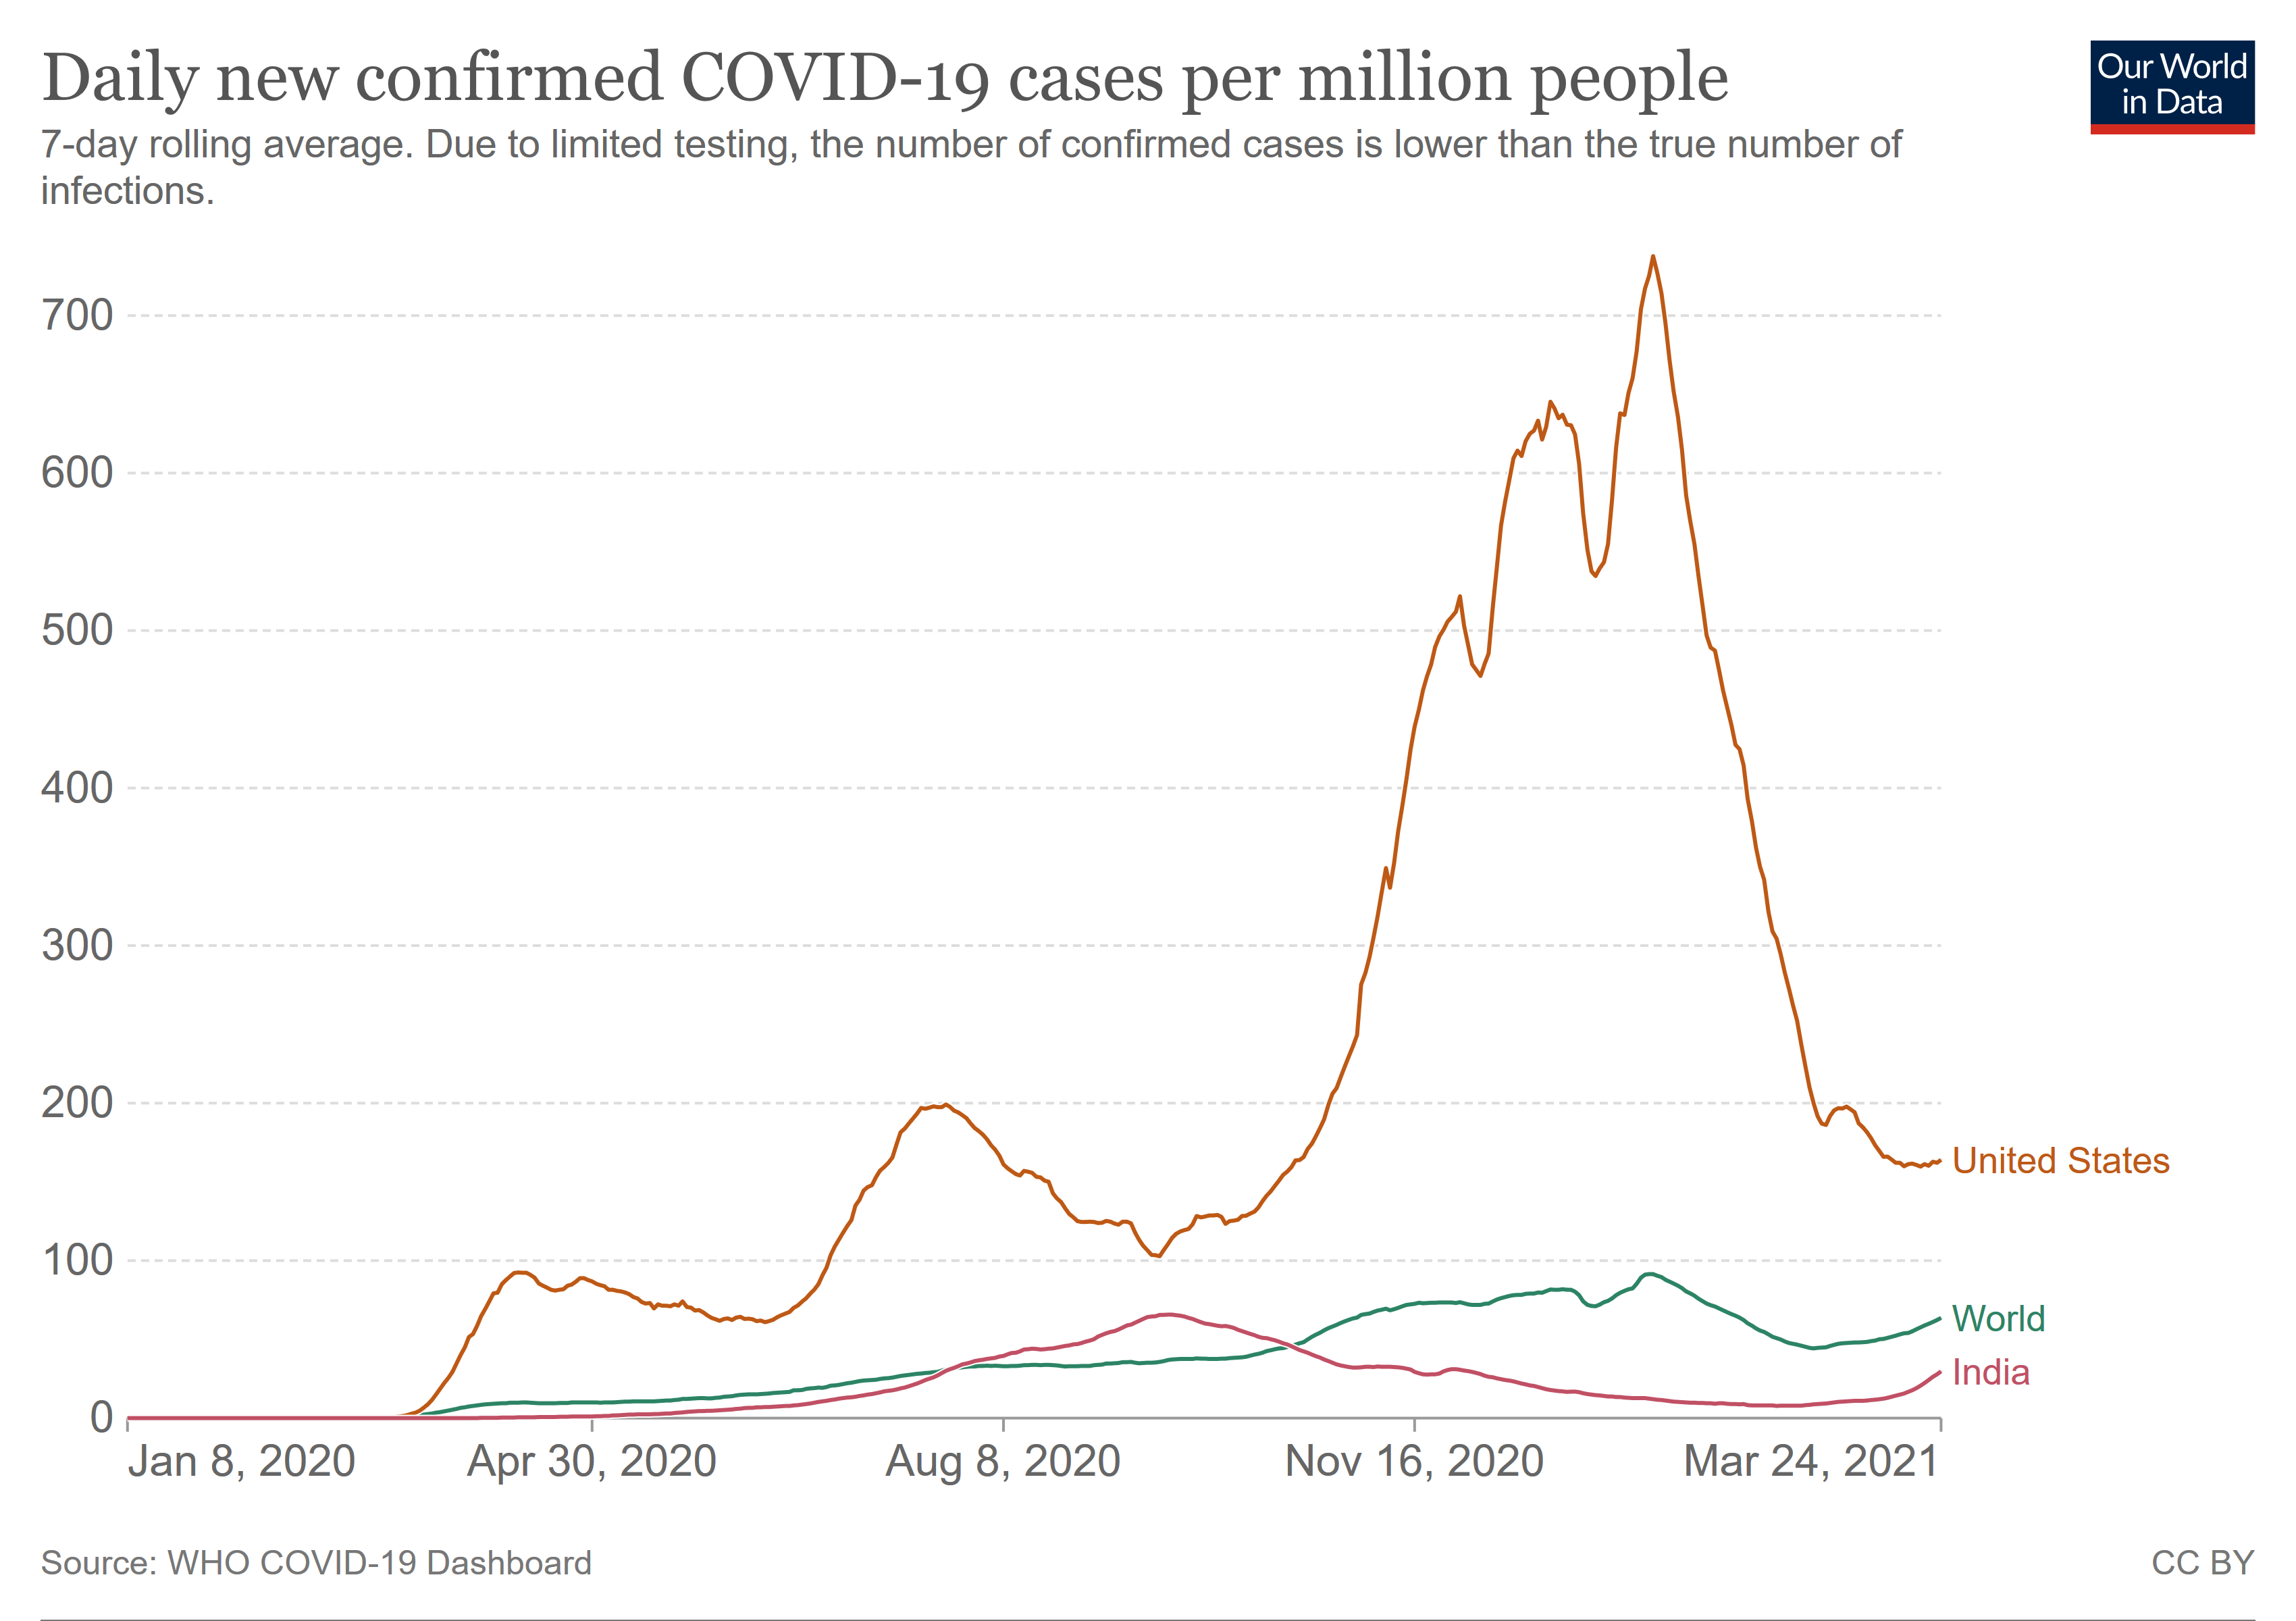
\includegraphics[width=1\linewidth]{confirmedCases}
\caption{ \label{fig:confirmedCases}}
\end{subfigure}
\begin{subfigure}{.49\textwidth}
\centering
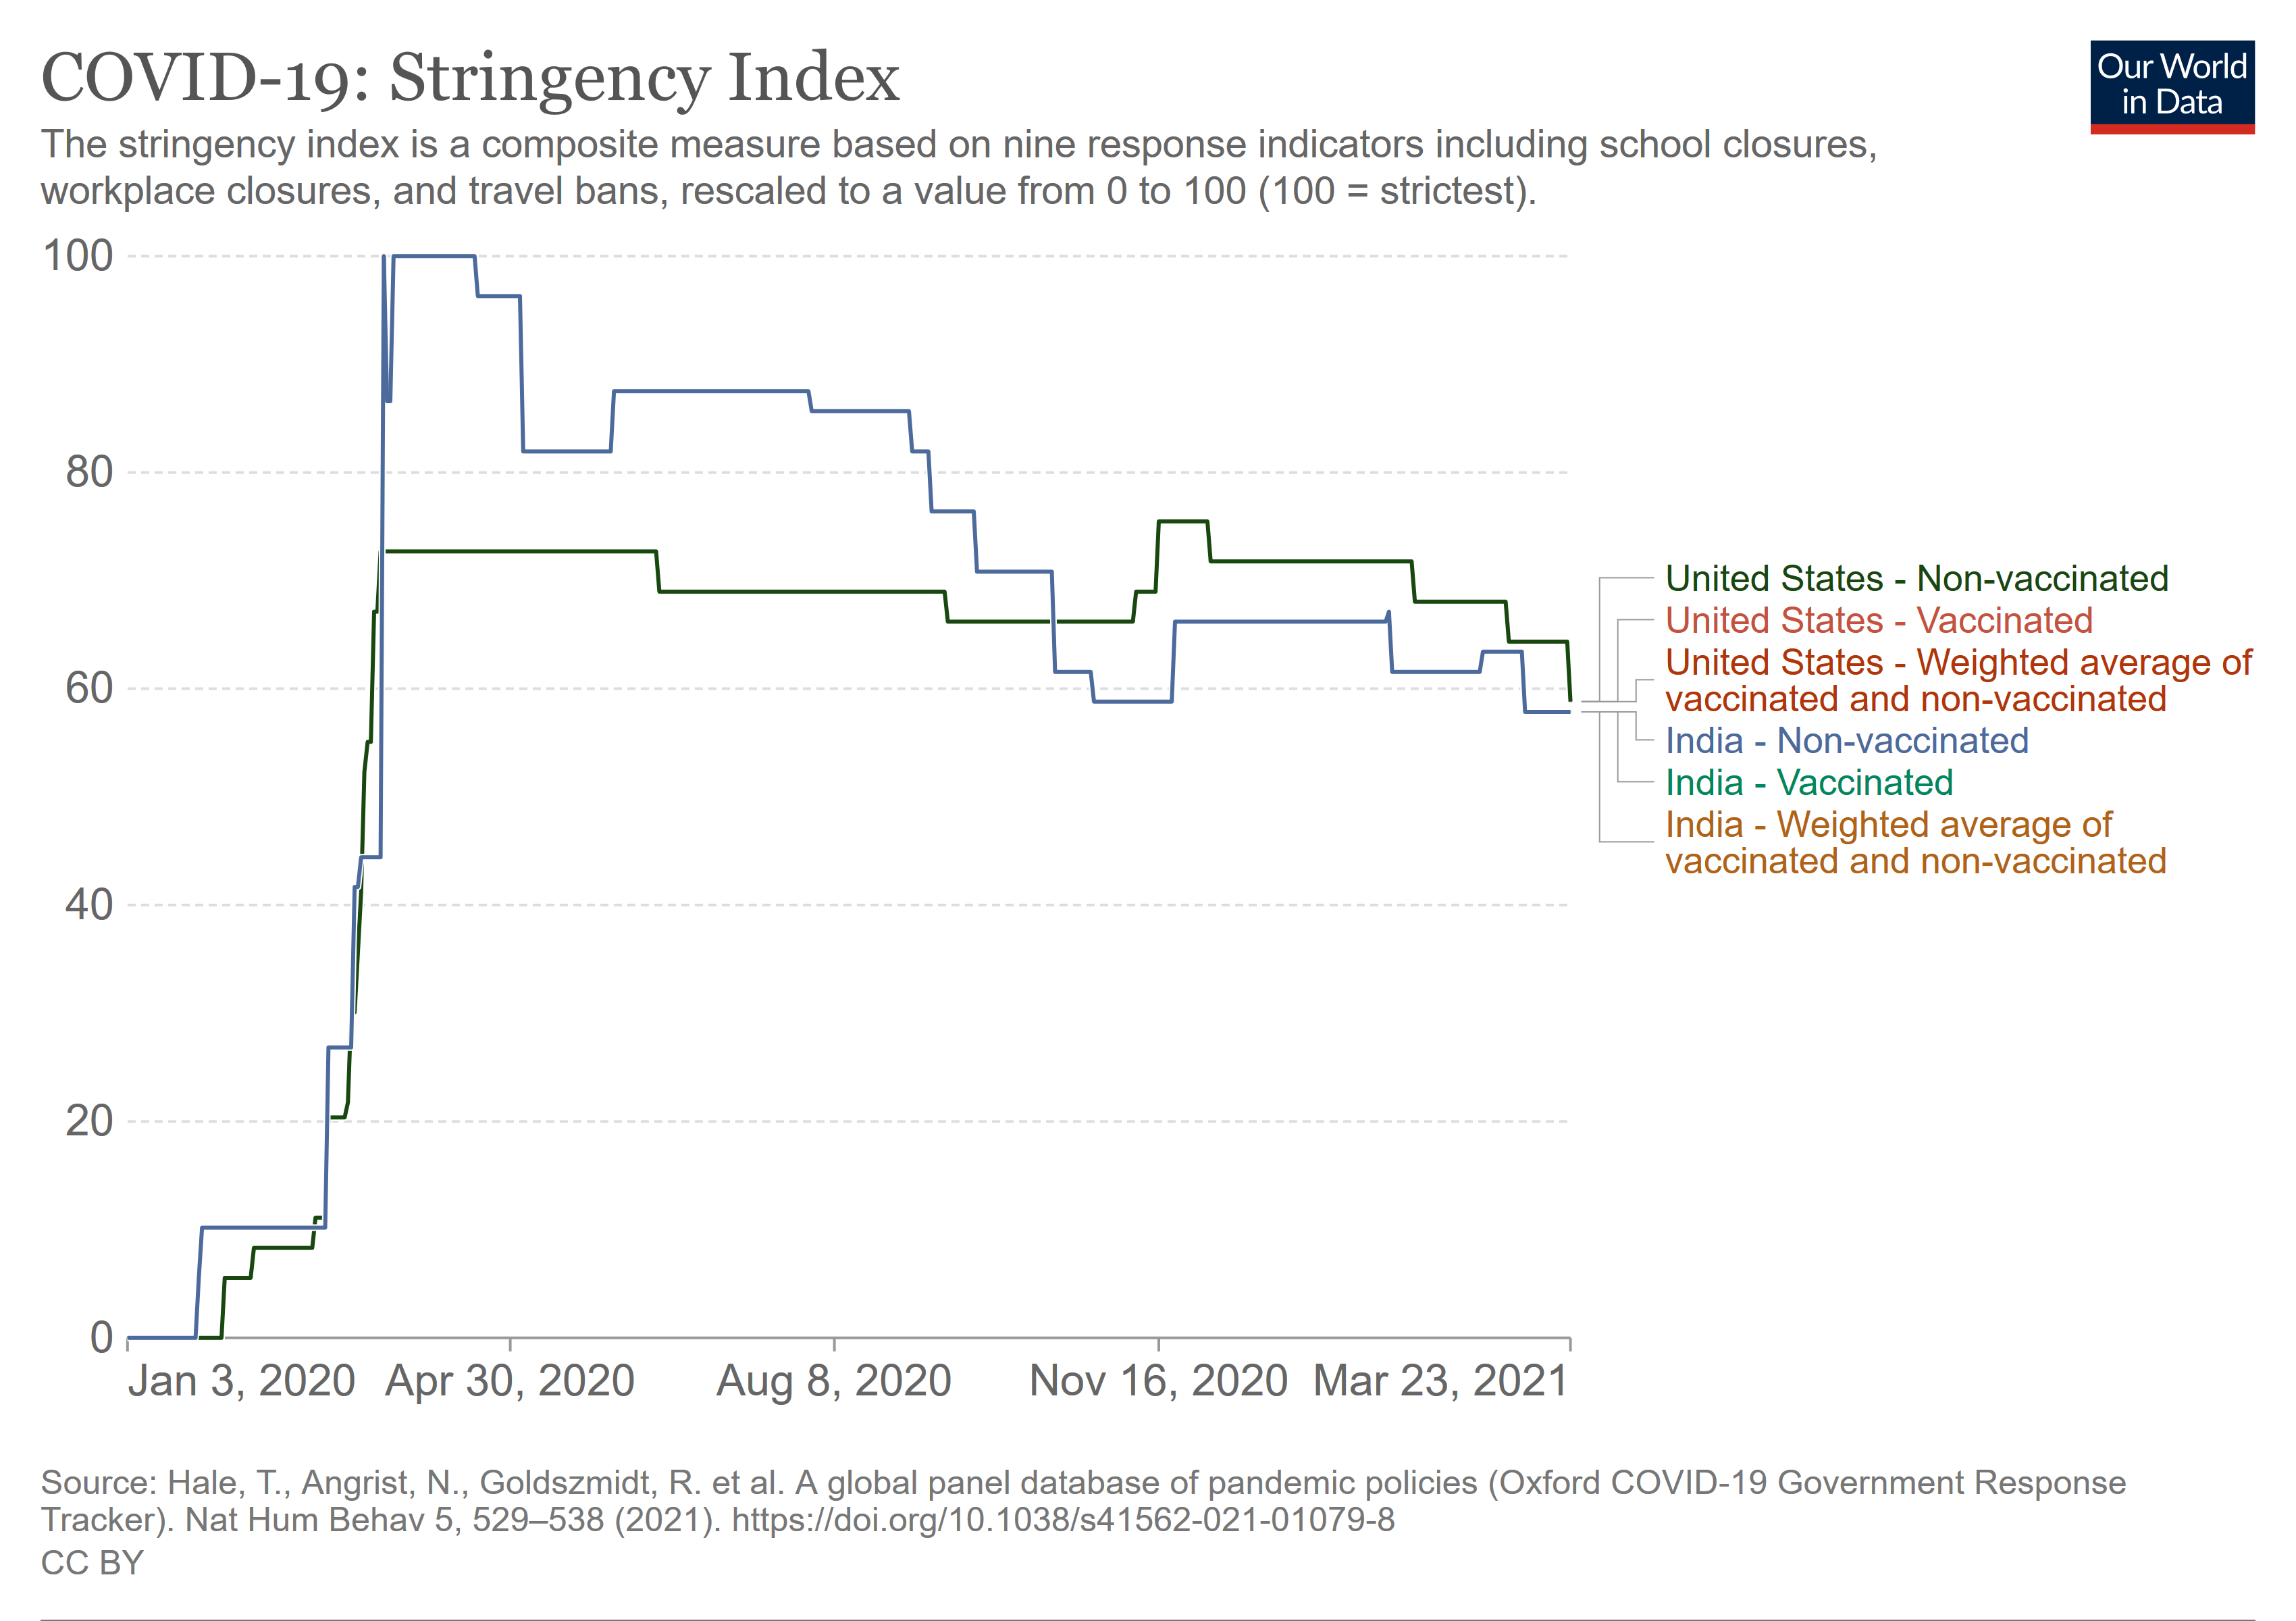
\includegraphics[width=1\linewidth]{stringency}
\caption{ \label{fig:stringencyCases}}
\end{subfigure}
\caption{\label{fig:indiaCovid} (a) Number of daily confirmed COVID-19-cases per million people for India, United States, and world average. X-axis covers the dates used in the main analysis of this work. (b) COVID-19 stringency index (ref. \cref{subsec:stringencyData} for the details of index calculation) for the same countries. (\citet{Mathieu2020})}
\end{figure}

India is used as an empirical case. There are several reasons for this choice. First, India is the largest developing country with a population of over 1.4 billion in 2021\footnote{\url{https://data.worldbank.org/indicator/SP.POP.TOTL?locations=IN}, United Nations Population Division. World Population Prospects: 2022 Revision, cited 2023-5-13}. Therefore, its sole contribution is already significant. Although the results are predictive and hence indicative, \citet{Lakmer:2022} argue in their 2020 poverty estimates that the predicted decrease was indeed driven by India. Second, the direct health effects of COVID-19 infection were relatively mild in India during the first wave of the pandemic, but the government responses in terms of practiced policies were still very stringent. The former is visualized in \cref{fig:confirmedCases}, which shows the daily new confirmed COVID-19 cases of India with respect to the United States and world average, and the latter in \cref{fig:stringencyCases} showing the stringency of the policies for the same inputs. This makes it possible to separate indirect health effects from direct ones in India during first wave of COVID-19 pandemic. Third, DHS data collection was in progress in India when the first wave of COVID-19 spread worldwide on spring 2020, which means there are good data available for the purpose.

The study is important because the COVID-19 pandemic was a unique shock, the likes of which has not been experienced in the last hundred years. Therefore, it is important to know and understand the implications that the practiced policies may have caused. Investigating potential changes in health outcomes is a key step toward such an understanding.

The rest of this thesis, after this introductory \cref{sec:introduction}, is organized as follows. The background and related literature from the connection between health and economic outcomes are presented in \cref{sec:literature}, including the background for selected health outcomes that are used later in this work. Thereafter, used empirical approach is presented in \cref{sec:empirical}: used DHS data in \cref{subsec:data}, used model in \cref{subsec:model}, selected health outcome variables -- along with detailed analysis for some of them -- in \cref{subsec:outcomeVariables} and conducted balancing checks for the used data in \cref{subsec:balancing}. Results of main analysis are shown in \cref{subsec:results}: for vaccination, nutrition, and rest of the outcomes the results are shown in \cref{subsec:resultsVaccination,subsec:resultsNutrition,subsec:resultsOtherOutcomes}, respectively, which is then followed by presenting additional considerations, validations, and robustness checks in \cref{subsec:additionaltests}. To further explore the possible effects in practiced policies, an additional stringency analysis is run as well in this thesis. It is presented in \cref{sec:stringency}: used data, used model, and corresponding results are presented in \cref{subsec:stringencyData,subsec:stringencyModel,subsec:stringencyResults}. All the results of this thesis are further discussed in \cref{sec:discussion}, mostly examining them considering recent literature. The thesis is finally concluded in \cref{sec:conclusion}.

\newpage
\section{Health and Economic Development} \label{sec:literature}

The global Multidimensional Poverty Index\footnote{\url{https://ophi.org.uk/multidimensional-poverty-index/}, cited 2023-5-13 (\citet{Alkire:2022})} is a standard used for measuring global poverty. Along with education and living standards, health is one of the three main pillars used to calculate the index. Why is that? In particular, why would an economist be interested in health and health outcomes?

Health may influence a country's economic development through several channels. \citet{Weil2007} classifies these channels into proximate and indirect ones. The proximate channel is a direct one: if an individual is healthy, she is simply a better worker and thus both productivity and working hours are higher.

In addition to proximate channels, \citet{Weil2007} lists several indirect channels. If health is improved, the level of education is also improved, as the investments needed to acquire schooling may be better compensated in the long run, which in turn will boost investments in schooling. In addition, healthy students are better in terms of cognitive functioning and attendance rate, which increases the effective education level per hours of education. Education being one of the most important prerequisites for economic development (e.g., \citet{Schultz:1961}), this channel is of high significance in terms of economic development.

\citet{Weil2007} continues listing the indirect channels with the increase in investments and savings for retirement. If health is improved, so does mortality, which furthermore stimulates these investments and savings since they are better paid off. This, in turn, will further increase the total and \textit{per capita} levels of investments and physical capital. An increase in the marginal product of capital, supported by the increased labor input of healthier workers, potentially has a similar effect.

Therefore, it is evident that health plays an important role as the basis of overall economic development. For this reason, it should also be of interest to an economist who wants to understand the foundations of economic development, as well as related policy implications.

In addition to these general health effects of any country or jurisdiction, \citet{Dupas:2011} presents two specific features that are typical of developing countries. First, there exists a high spending on curative care. Together with low fiscal support from government, it means that citizens have high "out-of-pocket" costs on health. Second, and in contrast, there is low spending on preventive care. This is potentially one of the reasons for the slow economic growth in developing countries, as focusing more on preventive care is in many cases more cost-effective, and thus the resources that are spent on curative care instead, could have been used for other purposes.

Due to the nature of the complex interrelated mechanisms and potentially very long-term effects, it is challenging to investigate the relationships between health and subsequent economic development, and specifically to show whether such a relationship is causal or not. They evidently affect each other as well and are also affected by other factors that are not easy to measure. Despite this endogeneity, there does exist literature in which different health outcomes are used as a measure for the purpose.

In the following sections, a set of health outcomes are briefly presented, as well as examples on how they have been used as health measure in terms of later economic development. Similar outcomes will be used later in this study (\cref{subsec:outcomeVariables}). All the selected health outcomes have in common that they can be influenced as well as addressed with appropriate policies.

\subsection{Immunization}

Immunization coverage and related vaccination in general are one of the most important factors in improving health both at the level of the individual and the population. After conducting a systematic review on economic benefits of vaccinations, \citet{Ozawa:2012} state that while the effects on overall livelihoods and economic benefits are evident, the literature tends to be relatively narrow in its view when the benefits are quantified. \citet{Ozawa:2012} conclude that the focus has mostly been on direct and short-term savings in the form of avoiding certain diseases, and short- and long-term indirect effects have either not been considered at all, or their impact has not been quantified -- such as preventing delays in cognitive development which increases productivity later or preventing a lot of costs for medical care.

\citet{Atwood:2022}, however, have recently showed that with proper research design, it is indeed possible to investigate indirect long-term effects as well. In her paper, she provided evidence from a causal link from improved measles immunization in childhood gained with measles vaccine to increase in adulthood earnings. In the United States, the measles vaccines were first brought into use in 1963. \cite{Atwood:2022} utilizes two different sources of variations in her work. First, because there existed differences in population densities across the states the pre-vaccine measles incidence rates were differing a lot as well. Second, different cohorts of children were exposed to the measles vaccines for the different amount of time, depending on children's month of birth. These allowed her to build a differences-in-differences-model, which she then used to estimate the effect that proper measles vaccination have had on later human capital accumulation. She used lifetime earnings as a measure for human capital accumulation. The main result was that the increase in earnings was 1.1\% with better immunization -- more precisely, such an increase was estimated for an individual with full exposure to the measles vaccination in a state with an average pre-vaccine measles incidence rate, as compared to an individual with no exposure to the vaccination in same state. In addition, this increase seems to have been achieved in the form of increased productivity, instead of an increase in work hours, further emphasizing the effect of accumulating human capital.

\subsection{Malnutrition}

World Health Organization (WHO) defines malnutrition as deficiencies or imbalances of an individual's intake of energy or nutrients\footnote{\url{https://www.who.int/news-room/fact-sheets/detail/malnutrition} -- WHO Key Facts on Malnutrition, accessed on 2023-4-8}. They further classify it into three different categories according to the underlying conditions, namely into undernutrition -- which can be measured by stunting, wasting or underweight -- micronutrient-related malnutrition, and overweight, obesity or diet-related noncommunicable diseases. Since this thesis focuses on developing countries, the focus is accordingly only on undernutrition and micronutrient-related malnutrition.

A famous review between nutrition and economic outcomes was made by \citet{Strauss:1998}. While they mention the difficulties in investigating the existence of possible causal relationship, they emphasize its importance for further research, and provide guidance for conducting such studies, as well as evidence from the existing literature on the impact of malnutrition on later economic outcomes, such as productivity. However, most of the outcomes were not given a magnitude, only a direction. In the evidence authors present, weight, height, and the corresponding Body Mass Index (BMI) were used as a proxy to malnutrition.

In terms of micronutrient-related malnutrition, one of the biggest reasons is iron-deficient based anaemia. For this reason, \citet{Hunt:2002} presents several benefits to be received when addressing iron deficit issues: direct productivity growth as an immediate improvement in work capacity; an increase in indirect productivity in the form of improved cognitive abilities and achievements; saving deaths for both adult and especially children and increasing economic growth, mostly due to corresponding cost savings. 

\citet{Chong:2016} conducted a study to investigate the effect of reduced iron deficiency on human capital accumulation, which they measured using both cognitive tests and school grades as well. They built up a Randomized Controlled Trial (RCT) among students in Cajamarca, rural Peru. The treatment groups were provided by additional iron bills, with a randomly assigned type of incentive in taking them. The main result was that measured ten weeks after the start of iron bill supplementation efforts, the cognitive ability, measured by scores from certain cognitive test, was increased by 21\% among students who were anaemic at baseline, whereas no change was measured among students who were not anaemic at baseline. In addition, this seemed to carry over to school performance as well, since the grades from corresponding academic year were increased by 0.45 (grading scale 0 to 5) among students who were anaemic at baseline, again with no change among students who were not. \citet{Chong:2016} concluded that the barrier that iron deficiency may cause on human capital accumulation is potentially a significant barrier to later economic development as well.

\subsection{Alcohol abuse and smoking}

By default, the societal costs of alcohol and smoking could be assumed to be obvious and significant. However, the actual assessment or estimation of such costs is extremely difficult -- for example, how to value lost years or years with disease burden, which may be shorter or longer, or how to account for taxation? However, the direct health effects on individuals are evident and can be both assessed and measured. For example, \cite{Griswold:2016} showed that alcohol use causes nearly 10\% of global deaths among population aged 15-49 years. Furthermore, \cite{Jha:2014} showed that smokers in low- and middle-income countries lose an average of ten years of life expectancy compared to non-smokers. In addition, the decrease in living standards increases along with the increased disease burden of both substances.

\citet{Schilbach:2019} recently conducted an interesting study to investigate the economic implications for individuals suffering from heavy alcohol consumption in developing countries. His starting point is the plausible assumption that excessive alcohol consumption has direct effects on health and self-control, which can then further affect productivity, savings, labor supply, and human capital investments. This, in turn, may reduce earnings and wealth, which furthermore may deepen poverty. Although plausible, there is no real evidence of the extent to which such economic effects exist -- if exist at all. \citet{Schilbach:2019} investigates this in field experiments of 229 male cycle-rickshaw drivers in Chennai, India, where heavy drinking is an issue among low-income workers. Using RCT and providing some of the participants with financial incentives for sobriety, he investigated, including quantitatively, how sobriety affects labor supply, productivity, earnings, and savings. According to his results, financial incentives caused participants to drink significantly less daily. Nevertheless, this had no effect on overall alcohol consumption. Somewhat surprisingly, his results showed that sobriety, however, did not significantly increase earnings or labor supply. Sobriety, however, increased savings considerably, by 50\%, and these savings were not fully accounted for by the change in income minus alcohol expenditures. His interpretation is that results suggest sobriety clearly improves forward-looking behavior and decision-making.

\subsection{Domestic violence}

Because there are so many reasons, manifestations and consequences of domestic violence, its effects on economic outcomes are exceptionally difficult to measure. However, as \citet{Krug:2002} points out, "victims of violence are at risk of psychological and behavioural problems, including depression, alcohol abuse, anxiety, and suicidal behaviour, and reproductive health problems, such as sexually transmitted diseases, unwanted pregnancies, and sexual dysfunction". The indirect effects of such consequences are evident and considerable.

\newpage
\section{Empirical approach} \label{sec:empirical}

\subsection{Data} \label{subsec:data}

Demographic and Health Survey (DHS) is the largest program that systematically and regularly collects nationally representative data on population, health, and nutrition in developing countries. DHS was launched in 1984, and since then more than 400 surveys have been conducted in more than 90 countries\footnote{\url{https://dhsprogram.com/}, cited on 2023-5-12}. In addition to the basic survey type, there are several other survey types tailored to the needs of each country, such as malaria indicator and service provision assessment surveys. The data is collected at both the household and individual level. In India, DHS surveys have been conducted since 1992, with a total of five survey rounds. In this thesis, the three most recent of them are used, with the focus being on the fifth, which is the most recent survey.

Fifth Demographic and Health Survey (DHS-5) was conducted in India between June 2019 and May 2021. The actual data collection was organized as National Family Health Survey (NFHS-5) of India, hosted by International Institute of Population Sciences (IIPS) and ICF International (\citet{iips2021}). Originally the data collection was supposed to be finished by the end of 2020. However, with the onset of the COVID-19 pandemic, India imposed complete lockdowns on spring 2020. Thus, the data collection process was stopped unexpectedly and unpredictably on March 22, 2020, and it was continued the following October, approximately half a year later. This break in data collection is utilized in this work, by comparing before and after break outcomes.

India has a total of 36 states. In DHS-5, there were in total 636726 household-level observations. In 13 of 36 states, data collection was in progress when it had to be stopped in March 2020, due to the restrictions. The data from these 13 states account for 51.6\% (328384 / 636726) of all household-level observations. Furthermore, 59.9\% (196632 / 328384) of the data from these 13 states were collected after the forced break. Therefore, unplanned, and unexpected break coincidentally provided a good setup for investigating the effects on health outcomes. In addition, only the observations from the same time window between January 7\ts{th} and March 20\ts{th} in consecutive years are included in the main analysis. This is done to minimize potential seasonal effects on result, as is further discussed in \cref{subsubsec:yearlyTrends}.

A histogram of DHS-5-data is shown in \cref{fig:dhsHistogram}, with red and blue box showing the time windows that are used in this thesis. All the corresponding observations are visualized in \cref{fig:india_areas}.

The previous DHS surveys of India, DHS-3 and DHS-4 were collected in 2005-6 and 2015-16. This thesis uses data also from DHS-3 and DHS-4, when investigating how the trends have evolved (\cref{subsubsec:trends}). While the data from the rest of the states -- more specifically, from those 23 states where data collection had already been finished on March 2020 -- is not used in the main analysis, which is fully based on DHS-5, it is nevertheless used as a reference data when investigating the past trends.

For individual level survey in DHS-5, there were a total of 765034 women and 124621 men aged 15-49 years surveyed, as well as 224349 children aged under five years. In addition, there were separate sub-modules for specific topics, such as violence, in which not all respondents participated. Therefore, sample sizes may differ across used health outcomes. DHS provides importance weights that are used in this thesis to balance possible differences in selection probability and interview between cases in used sample\footnote{\url{https://dhsprogram.com/data/Guide-to-DHS-Statistics/Analyzing_DHS_Data.htm}, cited on 2023-2-20}.

\begin{figure}
\begin{subfigure}{.49\textwidth}
\centering
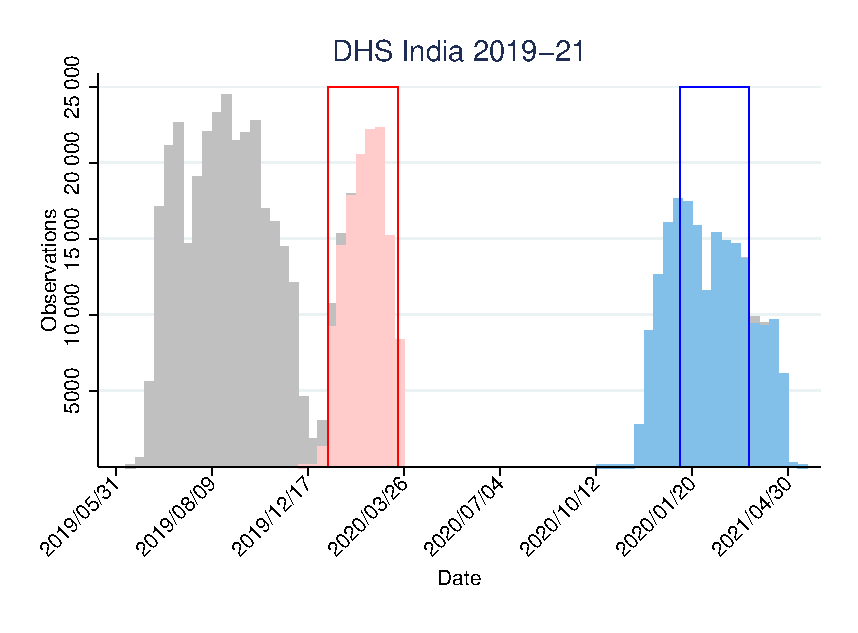
\includegraphics[width=1\linewidth]{dhsHistogram}
\caption{ \label{fig:dhsHistogram}}
\end{subfigure}
\begin{subfigure}{.49\textwidth}
\centering
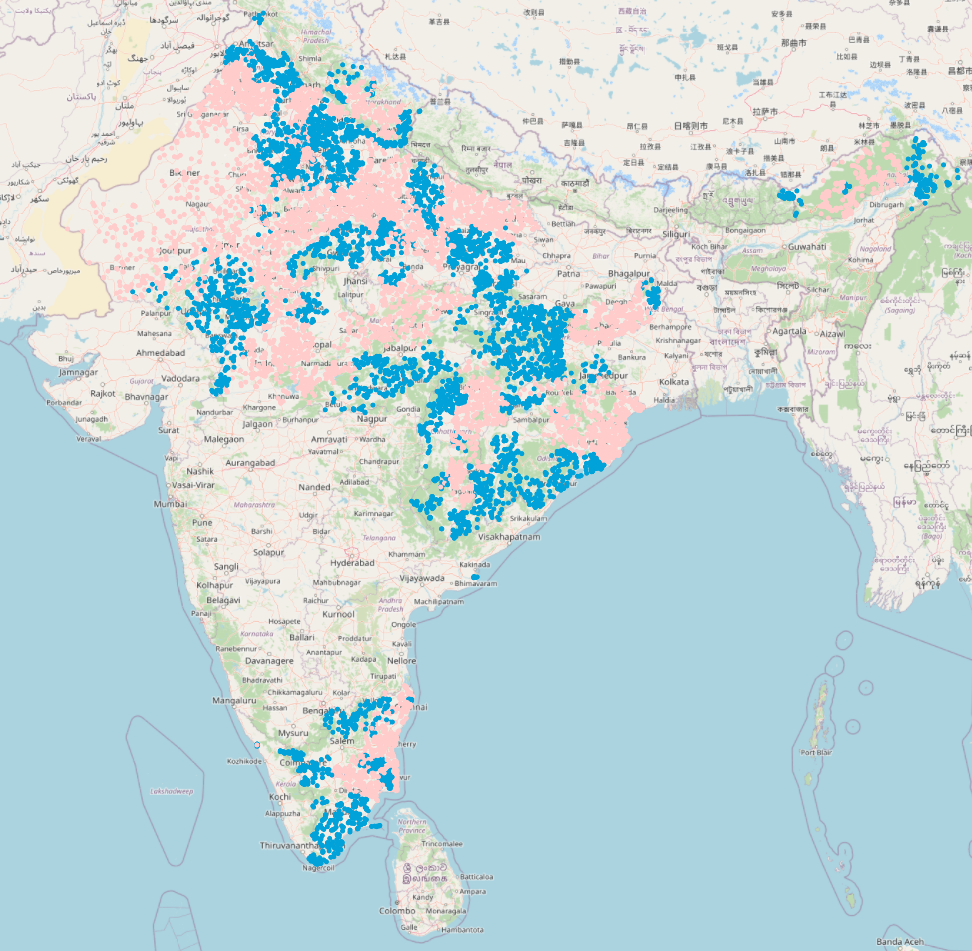
\includegraphics[width=1\linewidth]{allDataWinterMonthsLight}
\caption{ \label{fig:india_areas}}
\end{subfigure}
\caption{\label{fig:examples} (a) Data collection date histograms for the fifth India DHS survey for the entire country. Light red and light blue represent observations before and after March 2020, respectively, for \textit{in-progress} states. Light gray represents observations from \textit{reference} states. Red and blue boxes are used to visualize the time windows of equal width used between January 7\ts{th} and March 20\ts{th} of 2020 and 2021, respectively. All observations from \textit{in-progress} states within this window are included in the main analysis. (b) All observations from valid windows in (a) for \textit{in-progress} states, using the same coloring as in (a). \href{https://www.openstreetmap.org/copyright}{OpenStreetMap} is used as a background map.}
\end{figure}

As described in \cref{subsec:model}, wealth information is used also as a variable of interest. DHS does not provide direct income information. However, a specific wealth index has been derived from all wealth-specific data that DHS collects (\citet{DhsWealth:2004}). According to this wealth index, each interviewee can be classified into one of the following quintiles: Poorest, Poorer, Middle, Richer, Richest. This wealth index data is used in the main analysis of this thesis.

Considering the method used in this thesis, the order in which the sites are visited within the districts is important information. If there was some systematic order, it might affect the results and conclusions. Chapter "1.8 Strategy to ensure data quality" of \citet{iips2021} mentions that in each state, fieldwork was conducted in a group of five adjacent district at a time. The reason for this was logistical. However, there is no information about the order of sub-district visit. Randomization of the order would be optimal from a statistical point of view but considering that there is no evidence on the document of such randomization, and considering how much effort is required to organize the data collection, it is reasonable to assume that the order of the visits was not random, but instead optimal for each area from a logistical point of view. This is good to keep in mind when looking at the results.

Henceforth, \textit{before-} and \textit{after-lockdown} is used in this thesis as a term to describe the main division point of interest, which is March 22, 2020. For example, if the data is collected before March 22, 2020, the term \textit{before-lockdown} is used, and if after, the term \textit{after-lockdown} is used. Furthermore, terms \textit{reference} and \textit{in-progress} are used to refer states where data collection was either finished or in progress on March 22, 2020, respectively.

\subsection{Model} \label{subsec:model}

The aim of this thesis is to investigate possible changes in health outcomes that have happened during the COVID-19 pandemic, potentially as indirect consequences of applied strict policies. The main interest variable is thus the date of interview in terms of the COVID-19 onset. In addition, wealth information is used as another variable of interest in main analysis. The reason for including wealth information as an interest variable is that there are several potential reasons that may have affected differently high-wealth individuals or households, as compared to low-wealth ones. As an example, like discussed in \cref{sec:literature}, it is characteristics for individuals of developing countries to pay health costs out of pocket. As the lockdowns potentially caused job losses, high-wealth individuals might have been able to use their savings for health costs, even if they might have lost their jobs. That might not have been the case for low-wealth individuals, who may have been forced to avoid all the healthcare costs by avoiding visiting healthcare centers whatsoever, which thus might have intensified certain health deficiencies among low-wealth individuals. Similarly, they might not have had enough buffer to compensate possible income losses, and thus they may have had to settle for nutritionally poor or insufficient daily food.

For continuous health-specific outcome $h$, used model is therefore expressed as

\begin{equation} \label{eq:continuousModel}
\begin{split}
    Y_{ijk}^h = & \alpha^h + \beta_{1}^h After_i + \beta_{2}^h After_i \times LowWealth_i + \gamma^h LowWealth_i + \delta^h X_i +\\
    & State_j^h + Month_k^h + \varepsilon_{ijk}^h,
\end{split}
\end{equation}
%
where $Y_{ijk}^h$ is the outcome variable of interest of respondent $i$ from state $j$, surveyed in month $k$. $\beta_1^h$ and $\beta_2^h$ are the estimates of interests -- whether there have been changes since the start of the COVID-19-pandemic, and whether potential changes are specific for low-wealth individuals. $After_i$ and $LowWealth_i$ are indicator variables: $After_i$ equals 1 if the respondent was surveyed after March 22, 2020, and $LowWealth_i$ equals 1 if the state-specific wealth index of survey respondent $i$ belongs to first- or second-lowest wealth quintiles. $State_j$ is the state-specific fixed effect, and $Month_k$ is the month-specific fixed effect, related to the month of interview. $X_i$ is a vector of individual covariates: living in urban or rural areas; sex; age; month of birth, available only for child-specific outcomes; ethnicity -- a separate dummy variable of belonging to a scheduled caste or scheduled tribe; and religion -- a separate dummy variable for being Hindi, Muslim, Christian or Sikh. Age is a dummy variable per month for children, and per year for adults (see \cref{subsubsec:nutrition} for details when controlling for age). Testing for balancing of covariates used for data collected before and after the disruption due to COVID-19 are run prior to the main analysis, as discussed in more detail in \cref{subsec:balancing}.

\citet{Jakiela:2019} use a similar model as a first identifications strategy when they take advantage of an unplanned interruption of a longitudinal survey, caused by a violent post-election crisis, to measure the effect of violence on individual risk preferences.

Most dependent variables that are used in this thesis are binary random variables. Thus, a probit response model is used for such variables, estimating the conditional probability that $Y_{ijk}^h=1$, given the explanatory variables. It is written, analogously to \cref{eq:continuousModel}, as

\begin{equation} \label{eq:probitModel}
\begin{split}
    Pr(Y_{ijk}^h = 1) = &\Phi(\alpha^h + \beta_{1}^h After_i + \beta_{2}^h After_i \times LowWealth_i + \gamma^h LowWealth_i + \\
    & \delta^h X_i + State_j^h + Month_k^h),
\end{split}
\end{equation}
%
where the probit marginal effects $\beta_{1}^h$ and $\beta_{2}^h$ are the effects of interest.

A similar probit model is used by \citet{Bassi:2017} when they measure the causal impacts that persuasion potentially have had on fertility outcomes, using DHS data as well. Their approach is further discussed in \cref{subsec:limitations}, with respect to the approach used in this work.

In both \cref{eq:continuousModel} and \cref{eq:probitModel}, standard errors are clustered over districts.

\subsection{Outcome variables} \label{subsec:outcomeVariables}

The selection of health outcome variables of interest was done following certain guidelines. First, the outcomes that are shown to be either in a causal relationship, or at least in connection with the later economic outcomes are preferred. Second, such outcomes are also considered, which might theoretically serve as a proxy of underlying possible major changes, such as changes in the public health sector. In addition, an outcome needs to be at least theoretically measurable within one year. In total, 14 outcome variables were constructed from the survey data for further analysis. In addition to this main analysis, a separate detailed analysis is performed for vaccination- and nutrition-specific outcomes (\cref{subsubsec:detailedAnalysis}).

Some outcome variables are gender-specific (violence, alcohol, smoking). This is for a reason. Women are the main direct victims of domestic violence. On the other hand, smoking and alcohol consumption are very low among women in India, compared to men (\citet{iips2021}). Even though these outcomes are gender-specific, the potential consequences may affect the entire household, and thus the society as a whole in the long run.

The outcome variables are constructed in such a way that the direction of change is consistent. More specifically, if the estimate is positive, the realized change is expected to be worsened or deteriorated, and correspondingly, if the estimate is negative, the realized change is expected to be improved. Although the direction may seem a little unconventional for some health outcomes, the consistency achieved in the interpretation of the results compensates for the possible unconventionality in the interpretation of the result of individual health outcome.

\subsubsection{Vaccination} \label{subsubsec:vaccination}

Regarding vaccination-specific health outcomes, the official guidelines of \citet{who2019Vaccination} are used to construct the corresponding indicators.

\begin{itemize}
    \item \textbf{Child Is Not Fully Vaccinated:} The variable is constructed according to the \textit{Fully vaccinated (basic antigen) coverage indicator}-instructions. The indicator refers to the percentage of children who receive each recommended vaccine dose of six basic antigens given in eight vaccinations: one dose of Bacillus Calmette-Guérin (BCG), three doses of Diphtheria-Tetanus-Pertussis, three doses of polio, and one dose of measles containing vaccine (MCV). Missing values and \textit{don't know}-values are classified as not receiving corresponding vaccination, according to the recommendation. In addition, as recommended in the guidelines, only children aged 12-24 months are included to account for possible delayed vaccination. The variable gets value 0 if a child has received  all vaccinations, and 1 if one or more are missing.

    Only children aged 12-24 months are needed for establishing proper immunization coverage. However, given the approach of this work -- more specifically, including January-March observations from consecutive years to account for the potential impact of COVID-19 -- this may not properly capture the potential effect of interest. If the vaccination programs were working properly before potential (indirect) impact of COVID-19, it is expected that most children aged 12-24 months in January-March 2021, have received all vaccinations already before March 2020. To better capture changes from children who have theoretically been affected by measures related to COVID-19, children aged 1-12 months are separately investigated, in addition to children aged 12-24 months. It should be noted that this variable does not reflect true immunization coverage, but instead is included in the analysis to capture potential COVID-19-related changes.

    \item \textbf{Child Is Never Vaccinated:} As for the variable \textit{Child Is Not Fully Vaccinated}, this variable is constructed following the guidelines from \cite{who2019Vaccination} related to \textit{Never Vaccinated coverage indicator}. The variable gets value 1 if a child aged 12 to 24 months has none of the eight basic vaccinations, and 0 if she has one or more of them. Recommendations regarding age and missing values are followed in the same way as in \textit{Child Is Not Fully Vaccinated}.

    Like \textit{Child Is Not Fully Vaccinated}, this variable is calculated separately for children aged 1-12 months as well, in addition to children aged 12-24 months.
\end{itemize}

\subsubsection{Nutrition} \label{subsubsec:nutrition}

Regarding child-specific nutrition outcomes, Child Growth Standards published by the WHO in 2006 (\citet{world2006child}) are used to construct the corresponding indicators. DHS-specific guidelines\footnote{\href{https://dhsprogram.com/data/Guide-to-DHS-Statistics/Nutritional_Status.htm}{https://dhsprogram.com/data/Guide-to-DHS-Statistics/Nutritional\_Status.htm}, accessed on 2023-5-7}, which are based on the same standards, are also utilized.

\begin{itemize}
    \item \textbf{Child Stunting:} Child stunting is constructed from height\hyp{}for\hyp{}age\hyp{}z\hyp{}scores (HAZ): a child aged 0-5 years suffers moderate or severe stunting (1) if her HAZ-score is less than -2.0, and otherwise does not suffer (0). Stunting serves as a measure of chronic nutritional deficiency.

    As pointed out by \citet{Cummins2013}, using HAZ in a DHS-type survey can lead to model misspecification bias for cohort-level determinants when identification is based on spatio-temporal, annual or seasonal variation. Following the first proposal by \citet{Cummins2013}, this threat is addressed by controlling the age using a completely flexible form representation, i.e., employing age-in-month dummy variables into the model \cref{eq:probitModel}. In addition, the models are controlled for children birth of month.

    \item \textbf{Child Underweight}: Child underweight is constructed from weight\hyp{}for\hyp{}age\hyp{}z\hyp{}scores (WAZ): a child aged 0-5 years is moderately or severely underweight (1) if her WAZ-score is less than -2.0, and normal weight otherwise (0). Underweight serves as a composite measure of both acute and chronic nutritional statuses.

    \item \textbf{Child Wasting:} Child wasting is constructed from weight\hyp{}for\hyp{}height\hyp{}z\hyp{}scores (WHZ): a child aged 0-5 years suffers moderate or severe wasting (1) if her WHZ-score is less than -2.0, and otherwise does not suffer (0). A measure serves as a measure of acute nutritional deficiency.

    \item \textbf{Child Is Anaemic:} A child is anaemic (1) if her haemoglobin level (g/dl, adjusted for altitude) is less than 11.0, and otherwise she is  not anaemic (0).

    \item \textbf{Adult Underweight}: Adult underweight outcome variable is constructed from BMI: an adult is underweight (1) if her BMI is less than 18.5, and otherwise normal weight (0). Both men and women are used, but an observation is accepted only if an individual is at least 18 years old. In addition, women who were pregnant on the day of the interview or who had given birth in two months prior to the interview were also excluded.

    \item \textbf{Adult Is Anaemic:} An adult is anaemic (1) if the haemoglobin level (g/dl, adjusted for altitude and for smoking status, if known) is less than 11.0 or 13.0 for women and men, respectively, and otherwise non-anaemic (0).

\end{itemize}

\subsubsection{Alcohol and Smoking (Men)}  \label{subsubsec:alcoholSmoking}

\begin{itemize}
    \item \textbf{Men Use Alcohol}: A variable is constructed from survey question "Do you drink alcohol?", which is a part of the men's submodule only. Variable gets value 1 for \textit{yes}, and 0 for \textit{no}.

    \item \textbf{Men Do Smoke}: A variable is constructed from survey part "Smokes nothing" which is a part of the men's submodule only. Variables gets value 1 for \textit{no}, and 0 for \textit{yes}.
\end{itemize}

\subsubsection{Experience of domestic violence and Number of injections used (Women)} \label{subsubsec:violenceInj}

\begin{itemize}
    \item \textbf{Experienced Any Violence:} This outcome variable is constructed for individual women selected for the domestic violence submodule. The interviewee has experienced violence (1) if she has answered \textit{yes} to any of the following four questions:
    \begin{itemize}
        \item Experienced any emotional violence
        \item Experienced any less severe violence
        \item Experienced any severe violence
        \item Experienced any sexual violence
    \end{itemize}
    Otherwise, the variable gets value zero.
    \item \textbf{Number of Injections}: A variable is a continuous number of injections that an interviewee has received in the last 12 months. A question is part of the women's submodule only.
\end{itemize}

\subsubsection{Detailed analysis} \label{subsubsec:detailedAnalysis}

\begin{itemize}
    \item \textbf{Vaccination:} In addition to the immunization coverage-related indicators presented in \cref{subsubsec:vaccination}, a detailed analysis is performed separately for each common vaccination, namely BCG, DPT-1, DPT-2, DPT-3, Polio-1, Polio-2, Polio-3 and Measles. A variable gets value 1 if a child aged 12-24 months has not received the corresponding vaccination or if the status is missing or unknown, and 0 otherwise. Like in the main analysis, a detailed analysis is also performed separately for children aged 1-12 months.

    \item \textbf{Nutrition indicators:} To analyze nutrition statuses presented in \cref{subsubsec:nutrition} in more detail, breastfeeding and complementary feeding indicators are studied. This is done by constructing three different indicators according to WHO recommendations to assess infant and young child feeding practices (\citet{who2021FoodIndicators}). Corresponding guide for DHS statistics is also used\footnote{\url{https://dhsprogram.com/data/Guide-to-DHS-Statistics/Minimum_Dietary_Diversity_Minimum_Meal_Frequency_and_Minimum_Acceptable_Diet.htm}, accessed on 2023-5-7}. As recommended in the document, all three used indicators are constructed separately for breastfed and non-breastfed children aged 6 to 24 months.

    The rationale behind all the dietary indicators is similar: the lack in dietary diversity may raise the risk of micronutrient deficiencies, which can further negatively affect later physical and cognitive development. In addition, food group diversity has been shown to be positively associated with the linear growth of young children (\citet{who2021FoodIndicators}). Furthermore, less frequent feed meal intake can also compromise micronutrient and total energy intake, which may lead to new micronutrient deficiencies, growth faltering and stunting.

    \begin{itemize}
        \item \textbf{Minimum Dietary Diversity (MDD):} Dietary diversity is considered to meet the minimum requirements (0) for a child if, during the 24 hours before the time of survey, she has received food from at least five out of eight of the following food categories:
        \begin{itemize}
            \item Breast milk
            \item Grains, roots, tubers, and plantains
            \item Pulses, nuts, and seeds
            \item Dairy products
            \item Flesh foods\footnote{One of the three flesh food category, "\textit{Gave child meat}", is not collected in India DHS survey. Thus, status is constructed using only two variables, namely "\textit{Gave child liver, heart, other organs}" and "\textit{Gave child fish or shellfish}".}
            \item Eggs
            \item Vitamin-A rich fruits and vegetables
            \item Other fruits and vegetables
        \end{itemize}
        Otherwise, dietary diversity is classified as not meeting the minimum requirements (1). As explained in \citet{who2021FoodIndicators}, since 2017, the calculation of this figure is not different between breastfed and non-breastfed children. While the calculation doesn't differ, in this work the figure is still calculated separately for both groups.

        \item \textbf{Minimum Meal Frequency (MMF):} Meal frequency is considered to meet the minimum requirements (0) for a child if, within 24 hours before the time of survey,
        \begin{itemize}
            \item she is non-breastfed, and she has received at least four feedings of solid, semi-solid or soft foods or milk feeds, of which at least one feeds must be other than milk feed, or
            \item she is breastfed and
            \begin{itemize}
                \item she is 6-8 months old, and she has received at least two feedings of solid, semi-solid or soft foods, or
                \item she is 9-23 months old, and she has received at least three feedings of solid, semi-solid or soft foods.
            \end{itemize}
        \end{itemize}
        Otherwise, the meal frequency is classified as not meeting the minimum requirements (1).

        \item \textbf{Minimum Acceptable Diet (MAD):} Diet is considered as minimum acceptable (0) for a child if, within 24 hours before the time of survey,
        \begin{itemize}
            \item she is non-breastfed, and she has acceptable MDD and MMF, or
            \item she is breastfed, she has acceptable MDD and MMF, and in addition, at least two milk feeds\footnote{"Milk feeds include any formula or any animal milk other than human breast milk as well as semi-solid and fluid/drinkable yogurt and other fluid/drinkable fermented products made with animal milk." (\citet{who2021FoodIndicators})}.
        \end{itemize}
        Otherwise, MAD is considered not to be met (1).
    \end{itemize}

    Missing or invalid values are classified as zero for each of the three indicators.
\end{itemize}

\subsection{Balancing checks} \label{subsec:balancing}

The concern with the model used is the rather long time it takes for the data collection in general, but especially due to the pause caused by the COVID-19-induced lockdowns. There may be either timely trends or sampling strategical imbalances that could potentially affect the interpretation of the result. Addressing the former threat is covered in \cref{subsec:additionaltests}. In terms of the covariates used, the latter threat would be valid if, for some reason, there were proportionally significantly more (or fewer) observations of low-wealth individuals or from urban areas \textit{after-lockdown} than \textit{before-lockdowns}.

To address this threat, a test similar to \citet{Bassi:2017} is conducted: \textit{before}- and \textit{after-lockdown} proportions are calculated for all used covariates, and then the equality between the proportions is tested, using the sampling weights. The results of such tests are shown in \cref{tab:balanced,tab:balanced2,tab:balanced3,tab:balanced4}.

Regarding presumably the most important covariates, namely low-wealth- and region-status, equality tests for any of the outcome variables cannot be rejected, implying that these controls are balanced. The same is valid with sex, ethnic control, and most of the religion-dummies. Some of the religion dummies -- mainly "Is Hindi" -- have statistically significantly different mean values. However, while the difference is statistically significant, OLS, which is used in the test to be able to use DHS sampling weights, shows the difference is very small in magnitude, and therefore not relevant.

Equality tests for age show the balance for all other used outcomes except for nutrition-based health outcomes and number of injections. Interestingly, the differences are in the opposite direction when compared between children and adults: for \textit{Child Stunting}, \textit{Child Underweight}, \textit{Child Wasting} and \textit{Child Is Anaemic}, an average age is approximately 0.6 months less \textit{after-lockdowns}, as compared to \textit{before-lockdowns}, whereas for \textit{Adult Underweight}, \textit{Adult Is Anaemic} and \textit{Number of Injections}, an average age is approximately 0.2-0.3 years more for \textit{after-lockdowns}, as compared to \textit{before-lockdowns}. Although this imbalance must be kept in mind when interpreting the results, there are two things that mitigate any potential unwanted effects: First, as discussed in \cref{subsubsec:nutrition}, when age is used as a control for models presented in \cref{eq:continuousModel,eq:probitModel}, it is done using completely flexible form representation, namely employing age-in-month and -year as monthly and yearly dummy variables, respectively. Second, although the differences are statistically significant, they are relatively small economically.

\newpage

\section{Results} \label{subsec:results}

\begin{table}[htbp]\centering \footnotesize \renewcommand{\arraystretch}{0.3} \def\sym#1{\ifmmode^{#1}\else\(^{#1}\)\fi}\caption{\label{tab:tableLongProbit} \footnotesize Marginal probit estimates (\cref{eq:probitModel}) for vaccination-specific health outcome variables.}\begin{tabular}{lcccac} \hline\hline
                    &\multicolumn{1}{c}{(1)}         &\multicolumn{1}{c}{(2)}         &\multicolumn{1}{c}{(3)}         &\multicolumn{1}{c}{(4)}         &\multicolumn{1}{c}{(5)}         \\
\hline \\ \multicolumn{6}{l}{\textbf{Is Not Fully Vaccinated (12-24)}} \\\\[-1ex]
\textit{After}      &      -0.074\sym{***}&      -0.075\sym{***}&      -0.072\sym{***}&      -0.080\sym{***}&      -0.130\sym{***}\\
                    &     (0.015)         &     (0.015)         &     (0.015)         &     (0.015)         &     (0.027)         \\
[1em]
\textit{After} x \textit{LowWealth}&       0.005         &       0.006         &       0.004         &       0.010         &       0.087\sym{***}\\
                    &     (0.019)         &     (0.019)         &     (0.019)         &     (0.019)         &     (0.032)         \\
[1em]
Baseline High Wealth&       0.225         &       0.225         &       0.225         &       0.225         &       0.247         \\
Baseline Low Wealth &       0.280         &       0.288         &       0.289         &       0.286         &       0.296         \\
N                   &       16808         &       16808         &       16808         &       16633         &        5069         \\
R-Square            &       0.039         &       0.039         &       0.043         &       0.048         &       0.062         \\
\hdashline \\ \multicolumn{6}{l}{\textbf{Never Vaccinated (12-24)}} \\\\[-1ex]
\textit{After}      &       0.010\sym{**} &       0.010\sym{*}  &       0.010\sym{*}  &       0.007         &       0.005         \\
                    &     (0.005)         &     (0.005)         &     (0.005)         &     (0.005)         &     (0.012)         \\
[1em]
\textit{After} x \textit{LowWealth}&      -0.006         &      -0.006         &      -0.005         &      -0.003         &       0.005         \\
                    &     (0.007)         &     (0.007)         &     (0.007)         &     (0.007)         &     (0.014)         \\
[1em]
Baseline High Wealth&       0.022         &       0.022         &       0.022         &       0.022         &       0.025         \\
Baseline Low Wealth &       0.042         &       0.044         &       0.043         &       0.044         &       0.051         \\
N                   &       16687         &       16687         &       16687         &       16512         &        4961         \\
R-Square            &       0.023         &       0.024         &       0.036         &       0.047         &       0.084         \\
\hdashline \\ \multicolumn{6}{l}{\textbf{Is Not Fully Vaccinated (1-12)}} \\\\[-1ex]
\textit{After}      &      -0.014         &      -0.014         &      -0.019         &      -0.020         &      -0.026         \\
                    &     (0.015)         &     (0.015)         &     (0.014)         &     (0.013)         &     (0.022)         \\
[1em]
\textit{After} x \textit{LowWealth}&      -0.011         &      -0.011         &       0.000         &       0.003         &       0.003         \\
                    &     (0.020)         &     (0.020)         &     (0.017)         &     (0.017)         &     (0.033)         \\
[1em]
Baseline High Wealth&       0.537         &       0.537         &       0.537         &       0.536         &       0.531         \\
Baseline Low Wealth &       0.599         &       0.604         &       0.594         &       0.590         &       0.572         \\
N                   &       16260         &       16260         &       16260         &       16084         &        4873         \\
R-Square            &       0.023         &       0.023         &       0.306         &       0.307         &       0.300         \\
\hdashline \\ \multicolumn{6}{l}{\textbf{Never Vaccinated (1-12)}} \\\\[-1ex]
\textit{After}      &       0.011         &       0.011         &       0.010         &       0.008         &       0.043\sym{***}\\
                    &     (0.007)         &     (0.007)         &     (0.007)         &     (0.006)         &     (0.009)         \\
[1em]
\textit{After} x \textit{LowWealth}&       0.002         &       0.002         &       0.003         &       0.006         &      -0.028\sym{***}\\
                    &     (0.008)         &     (0.008)         &     (0.008)         &     (0.008)         &     (0.011)         \\
[1em]
Baseline High Wealth&       0.028         &       0.028         &       0.028         &       0.028         &       0.018         \\
Baseline Low Wealth &       0.046         &       0.052         &       0.051         &       0.049         &       0.054         \\
N                   &       16260         &       16260         &       16260         &       16084         &        4873         \\
R-Square            &       0.035         &       0.039         &       0.061         &       0.065         &       0.106         \\
\hline\\ State Fixed & \cmark & \cmark & \cmark & \cmark & \cmark \\ Region & \xmark & \cmark & \cmark & \cmark & \cmark \\ Time Controls & \xmark & \xmark & \cmark & \cmark & \cmark \\ Individual Controls & \xmark & \xmark & \xmark & \cmark & \cmark \\ \hline\hline \multicolumn{4}{l}{\footnotesize Standard errors in parentheses \Tstrut}\\ \multicolumn{2}{l}{\footnotesize \sym{*} \(p<0.1\), \sym{**} \(p<0.05\), \sym{***} \(p<0.01\)}\\ \end{tabular} \\ \caption*{\footnotesize \textbf{After} is the effect of after-lockdown-indicator, and \textbf{After x LowWealth} is the interaction between After and belonging to two lowest wealth quintiles. \textbf{Baseline High} and \textbf{Low Wealth} are before-lockdown-means of dependent variable of high and low wealth individuals, respectively. \textbf{Time Controls} are monthly or yearly dummies for month of interview, month of birth and age. \textbf{Individual Controls} include sex, ethnicity and religion background. In (5), observations are limited on intra-state edges only. DHS sampling weights are used, and standard errors are clustered over districts.} \end{table}

\begin{table}[htbp]\centering \footnotesize \renewcommand{\arraystretch}{0.3} \def\sym#1{\ifmmode^{#1}\else\(^{#1}\)\fi}\caption{\label{tab:tableLongProbit2} \footnotesize Marginal probit estimates (\cref{eq:probitModel}) for nutrition-specific health outcome variables.}\begin{tabular}{lcccac} \hline\hline
                    &\multicolumn{1}{c}{(1)}         &\multicolumn{1}{c}{(2)}         &\multicolumn{1}{c}{(3)}         &\multicolumn{1}{c}{(4)}         &\multicolumn{1}{c}{(5)}         \\
\hline \\ \multicolumn{6}{l}{\textbf{Child Stunting}} \\\\[-1ex]
\textit{After}      &      -0.017\sym{*}  &      -0.017\sym{*}  &      -0.017\sym{*}  &      -0.020\sym{**} &      -0.021         \\
                    &     (0.010)         &     (0.009)         &     (0.009)         &     (0.010)         &     (0.018)         \\
[1em]
\textit{After} x \textit{LowWealth}&       0.009         &       0.009         &       0.010         &       0.011         &      -0.002         \\
                    &     (0.011)         &     (0.011)         &     (0.011)         &     (0.011)         &     (0.018)         \\
[1em]
Baseline High Wealth&       0.300         &       0.300         &       0.300         &       0.301         &       0.304         \\
Baseline Low Wealth &       0.421         &       0.417         &       0.414         &       0.404         &       0.402         \\
N                   &       80224         &       80224         &       80224         &       79388         &       24243         \\
R-Square            &       0.025         &       0.025         &       0.041         &       0.044         &       0.050         \\
\hdashline \\ \multicolumn{6}{l}{\textbf{Child Underweight}} \\\\[-1ex]
\textit{After}      &      -0.024\sym{***}&      -0.024\sym{***}&      -0.023\sym{***}&      -0.028\sym{***}&      -0.018         \\
                    &     (0.008)         &     (0.008)         &     (0.008)         &     (0.008)         &     (0.013)         \\
[1em]
\textit{After} x \textit{LowWealth}&       0.021\sym{**} &       0.021\sym{**} &       0.021\sym{**} &       0.023\sym{**} &       0.003         \\
                    &     (0.010)         &     (0.010)         &     (0.010)         &     (0.010)         &     (0.016)         \\
[1em]
Baseline High Wealth&       0.250         &       0.250         &       0.250         &       0.250         &       0.251         \\
Baseline Low Wealth &       0.354         &       0.355         &       0.354         &       0.343         &       0.339         \\
N                   &       82137         &       82137         &       82137         &       81271         &       24857         \\
R-Square            &       0.023         &       0.023         &       0.028         &       0.031         &       0.034         \\
\hdashline \\ \multicolumn{6}{l}{\textbf{Child Wasting}} \\\\[-1ex]
\textit{After}      &      -0.034\sym{***}&      -0.034\sym{***}&      -0.036\sym{***}&      -0.038\sym{***}&      -0.022\sym{*}  \\
                    &     (0.008)         &     (0.008)         &     (0.008)         &     (0.007)         &     (0.012)         \\
[1em]
\textit{After} x \textit{LowWealth}&       0.012         &       0.012         &       0.012         &       0.012         &       0.011         \\
                    &     (0.009)         &     (0.009)         &     (0.009)         &     (0.009)         &     (0.016)         \\
[1em]
Baseline High Wealth&       0.170         &       0.170         &       0.170         &       0.169         &       0.164         \\
Baseline Low Wealth &       0.187         &       0.193         &       0.196         &       0.192         &       0.190         \\
N                   &       79231         &       79231         &       79231         &       78396         &       23931         \\
R-Square            &       0.008         &       0.008         &       0.024         &       0.025         &       0.033         \\
\hdashline \\ \multicolumn{6}{l}{\textbf{Adult Underweight}} \\\\[-1ex]
\textit{After}      &      -0.006         &      -0.007         &      -0.008         &      -0.008         &      -0.001         \\
                    &     (0.005)         &     (0.005)         &     (0.005)         &     (0.005)         &     (0.006)         \\
[1em]
\textit{After} x \textit{LowWealth}&       0.010         &       0.010         &       0.011\sym{*}  &       0.010         &       0.009         \\
                    &     (0.007)         &     (0.007)         &     (0.007)         &     (0.007)         &     (0.009)         \\
[1em]
Baseline High Wealth&       0.125         &       0.125         &       0.125         &       0.125         &       0.120         \\
Baseline Low Wealth &       0.210         &       0.199         &       0.200         &       0.195         &       0.190         \\
N                   &      259046         &      259046         &      259042         &      255908         &       80220         \\
R-Square            &       0.031         &       0.033         &       0.080         &       0.082         &       0.087         \\
\hline\\ State Fixed & \cmark & \cmark & \cmark & \cmark & \cmark \\ Region & \xmark & \cmark & \cmark & \cmark & \cmark \\ Time Controls & \xmark & \xmark & \cmark & \cmark & \cmark \\ Individual Controls & \xmark & \xmark & \xmark & \cmark & \cmark \\ \hline\hline \multicolumn{4}{l}{\footnotesize Standard errors in parentheses \Tstrut}\\ \multicolumn{2}{l}{\footnotesize \sym{*} \(p<0.1\), \sym{**} \(p<0.05\), \sym{***} \(p<0.01\)}\\ \end{tabular} \\ \caption*{\footnotesize \textbf{After} is the effect of after-lockdown-indicator, and \textbf{After x LowWealth} is the interaction between After and belonging to two lowest wealth quintiles. \textbf{Baseline High} and \textbf{Low Wealth} are before-lockdown-means of dependent variable of high and low wealth individuals, respectively. \textbf{Time Controls} are monthly or yearly dummies for month of interview, month of birth and age. \textbf{Individual Controls} include sex, ethnicity and religion background. In (5), observations are limited on intra-state edges only. DHS sampling weights are used, and standard errors are clustered over districts.} \end{table}

\begin{table}[htbp]\centering \footnotesize \renewcommand{\arraystretch}{0.3} \def\sym#1{\ifmmode^{#1}\else\(^{#1}\)\fi}\caption{\label{tab:tableLongProbit3} \footnotesize Marginal probit estimates (\cref{eq:probitModel}) for outcome variables.}\begin{tabular}{lcccac} \hline\hline
                    &\multicolumn{1}{c}{(1)}         &\multicolumn{1}{c}{(2)}         &\multicolumn{1}{c}{(3)}         &\multicolumn{1}{c}{(4)}         &\multicolumn{1}{c}{(5)}         \\
\hline \\ \multicolumn{6}{l}{\textbf{Child Is Anaemic}} \\\\[-1ex]
\textit{After}      &      -0.073\sym{***}&      -0.074\sym{***}&      -0.076\sym{***}&      -0.079\sym{***}&      -0.094\sym{***}\\
                    &     (0.011)         &     (0.011)         &     (0.011)         &     (0.011)         &     (0.016)         \\
[1em]
\textit{After} x \textit{LowWealth}&       0.004         &       0.004         &       0.003         &       0.000         &      -0.004         \\
                    &     (0.011)         &     (0.011)         &     (0.010)         &     (0.010)         &     (0.019)         \\
[1em]
Baseline High Wealth&       0.704         &       0.704         &       0.704         &       0.704         &       0.702         \\
Baseline Low Wealth &       0.744         &       0.742         &       0.748         &       0.737         &       0.725         \\
N                   &       71848         &       71848         &       71848         &       71120         &       21892         \\
R-Square            &       0.014         &       0.014         &       0.050         &       0.052         &       0.051         \\
\hdashline \\ \multicolumn{6}{l}{\textbf{Adult Is Anaemic}} \\\\[-1ex]
\textit{After}      &      -0.034\sym{***}&      -0.034\sym{***}&      -0.034\sym{***}&      -0.033\sym{***}&      -0.039\sym{***}\\
                    &     (0.009)         &     (0.009)         &     (0.009)         &     (0.009)         &     (0.012)         \\
[1em]
\textit{After} x \textit{LowWealth}&      -0.011         &      -0.010         &      -0.008         &      -0.013         &      -0.007         \\
                    &     (0.009)         &     (0.009)         &     (0.009)         &     (0.008)         &     (0.014)         \\
[1em]
Baseline High Wealth&       0.505         &       0.505         &       0.505         &       0.505         &       0.516         \\
Baseline Low Wealth &       0.558         &       0.550         &       0.550         &       0.540         &       0.552         \\
N                   &      271700         &      271700         &      271690         &      268600         &       84233         \\
R-Square            &       0.008         &       0.009         &       0.012         &       0.049         &       0.051         \\
\hdashline \\ \multicolumn{6}{l}{\textbf{Men Do Smoke}} \\\\[-1ex]
\textit{After}      &      -0.082\sym{***}&      -0.082\sym{***}&      -0.080\sym{***}&      -0.084\sym{***}&      -0.030         \\
                    &     (0.014)         &     (0.014)         &     (0.013)         &     (0.014)         &     (0.021)         \\
[1em]
\textit{After} x \textit{LowWealth}&       0.042\sym{**} &       0.042\sym{**} &       0.038\sym{**} &       0.040\sym{**} &      -0.004         \\
                    &     (0.018)         &     (0.018)         &     (0.017)         &     (0.017)         &     (0.024)         \\
[1em]
Baseline High Wealth&       0.440         &       0.440         &       0.440         &       0.441         &       0.432         \\
Baseline Low Wealth &       0.613         &       0.610         &       0.613         &       0.596         &       0.592         \\
N                   &       34863         &       34863         &       34863         &       34457         &       10426         \\
R-Square            &       0.081         &       0.081         &       0.129         &       0.135         &       0.156         \\
\hdashline \\ \multicolumn{6}{l}{\textbf{Men Use Alcohol}} \\\\[-1ex]
\textit{After}      &      -0.053\sym{***}&      -0.053\sym{***}&      -0.053\sym{***}&      -0.050\sym{***}&      -0.034         \\
                    &     (0.011)         &     (0.011)         &     (0.011)         &     (0.011)         &     (0.022)         \\
[1em]
\textit{After} x \textit{LowWealth}&       0.038\sym{***}&       0.038\sym{***}&       0.036\sym{***}&       0.029\sym{**} &      -0.003         \\
                    &     (0.013)         &     (0.013)         &     (0.013)         &     (0.013)         &     (0.026)         \\
[1em]
Baseline High Wealth&       0.234         &       0.234         &       0.234         &       0.235         &       0.263         \\
Baseline Low Wealth &       0.323         &       0.321         &       0.324         &       0.305         &       0.356         \\
N                   &       34863         &       34863         &       34863         &       34457         &       10426         \\
R-Square            &       0.062         &       0.062         &       0.091         &       0.107         &       0.104         \\
\hline\\ State Fixed & \cmark & \cmark & \cmark & \cmark & \cmark \\ Region & \xmark & \cmark & \cmark & \cmark & \cmark \\ Time Controls & \xmark & \xmark & \cmark & \cmark & \cmark \\ Individual Controls & \xmark & \xmark & \xmark & \cmark & \cmark \\ \hline\hline \multicolumn{4}{l}{\footnotesize Standard errors in parentheses \Tstrut}\\ \multicolumn{2}{l}{\footnotesize \sym{*} \(p<0.1\), \sym{**} \(p<0.05\), \sym{***} \(p<0.01\)}\\ \end{tabular} \\ \caption*{\footnotesize \textbf{After} is the effect of after-lockdown-indicator, and \textbf{After x LowWealth} is the interaction between After and belonging to two lowest wealth quintiles. \textbf{Baseline High} and \textbf{Low Wealth} are before-lockdown-means of dependent variable of high and low wealth individuals, respectively. \textbf{Time Controls} are monthly or yearly dummies for month of interview, month of birth and age. \textbf{Individual Controls} include sex, ethnicity and religion background. In (5), observations are limited on intra-state edges only. DHS sampling weights are used, and standard errors are clustered over districts.} \end{table}

\begin{table}[htbp]\centering \footnotesize \renewcommand{\arraystretch}{0.3} \def\sym#1{\ifmmode^{#1}\else\(^{#1}\)\fi}\caption{\label{tab:tableLongProbit4} \footnotesize OLS (\cref{eq:continuousModel}$^\dagger$) and marginal probit estimates (\cref{eq:probitModel}) for outcome variables.}\begin{tabular}{lcccac} \hline\hline
                    &\multicolumn{1}{c}{(1)}         &\multicolumn{1}{c}{(2)}         &\multicolumn{1}{c}{(3)}         &\multicolumn{1}{c}{(4)}         &\multicolumn{1}{c}{(5)}         \\
\hline \\ \multicolumn{6}{l}{\textbf{Experienced Any Violence}} \\\\[-1ex]
\textit{After}      &      -0.097\sym{***}&      -0.097\sym{***}&      -0.095\sym{***}&      -0.098\sym{***}&      -0.055\sym{**} \\
                    &     (0.013)         &     (0.013)         &     (0.012)         &     (0.012)         &     (0.022)         \\
[1em]
\textit{After} x \textit{LowWealth}&       0.027\sym{*}  &       0.027\sym{*}  &       0.024         &       0.024         &      -0.029         \\
                    &     (0.016)         &     (0.016)         &     (0.016)         &     (0.016)         &     (0.033)         \\
[1em]
Baseline High Wealth&       0.317         &       0.317         &       0.317         &       0.318         &       0.339         \\
Baseline Low Wealth &       0.398         &       0.395         &       0.396         &       0.382         &       0.445         \\
N                   &       23965         &       23965         &       23954         &       23691         &        7342         \\
R-Square            &       0.035         &       0.035         &       0.042         &       0.045         &       0.067         \\
\hdashline \\ \multicolumn{6}{l}{\textbf{Number of Injections$^\dagger$}} \\\\[-1ex]
\textit{After}      &      -1.092\sym{***}&      -1.085\sym{***}&      -1.090\sym{***}&      -1.077\sym{***}&      -1.061\sym{***}\\
                    &     (0.095)         &     (0.084)         &     (0.084)         &     (0.086)         &     (0.146)         \\
[1em]
\textit{After} x \textit{LowWealth}&      -0.290\sym{***}&      -0.295\sym{***}&      -0.320\sym{***}&      -0.324\sym{***}&      -0.157         \\
                    &     (0.104)         &     (0.095)         &     (0.094)         &     (0.094)         &     (0.168)         \\
[1em]
Baseline High Wealth&       2.863         &       2.863         &       2.863         &       2.873         &       2.868         \\
Baseline Low Wealth &       3.246         &       3.016         &       3.071         &       3.094         &       2.967         \\
N                   &      275055         &      275055         &      275055         &      271687         &       85585         \\
R-Square            &       0.016         &       0.019         &       0.025         &       0.026         &       0.029         \\
\hline\\ State Fixed & \cmark & \cmark & \cmark & \cmark & \cmark \\ Region & \xmark & \cmark & \cmark & \cmark & \cmark \\ Time Controls & \xmark & \xmark & \cmark & \cmark & \cmark \\ Individual Controls & \xmark & \xmark & \xmark & \cmark & \cmark \\ \hline\hline \multicolumn{4}{l}{\footnotesize Standard errors in parentheses \Tstrut}\\ \multicolumn{2}{l}{\footnotesize \sym{*} \(p<0.1\), \sym{**} \(p<0.05\), \sym{***} \(p<0.01\)}\\ \end{tabular} \\ \caption*{\footnotesize \textbf{After} is the effect of after-lockdown-indicator, and \textbf{After x LowWealth} is the interaction between After and belonging to two lowest wealth quintiles. \textbf{Baseline High} and \textbf{Low Wealth} are before-lockdown-means of dependent variable of high and low wealth individuals, respectively. \textbf{Time Controls} are monthly or yearly dummies for month of interview, month of birth and age. \textbf{Individual Controls} include sex, ethnicity and religion background. In (5), observations are limited on intra-state edges only. DHS sampling weights are used, and standard errors are clustered over districts.} \end{table}

\begin{table}[htbp]\centering \footnotesize \def\sym#1{\ifmmode^{#1}\else\(^{#1}\)\fi}\caption{\label{tab:analysisVaccDetailed} \footnotesize Marginal probit estimates (\cref{eq:probitModel}) for programme vaccinations}\begin{tabular}{l*{8}{c}} \hline\hline
                    &\multicolumn{1}{c}{BCG}&\multicolumn{1}{c}{DPT-1}&\multicolumn{1}{c}{DPT-2}&\multicolumn{1}{c}{DPT-3}&\multicolumn{1}{c}{Polio-1}&\multicolumn{1}{c}{Polio-2}&\multicolumn{1}{c}{Polio-3}&\multicolumn{1}{c}{Measles}\\
\hline \\ [-2em] \multicolumn{9}{l}{\textbf{Child 12-24 Months, Do Not Have Corresponding Vaccination}} \\
\textit{After}      &       0.005         &       0.006         &      -0.009         &       0.001         &      -0.027\sym{**} &      -0.012         &      -0.042\sym{***}&      -0.004         \\
                    &     (0.006)         &     (0.008)         &     (0.008)         &     (0.009)         &     (0.011)         &     (0.011)         &     (0.013)         &     (0.011)         \\
[1em]
\textit{After} x \textit{LowWealth}&      -0.005         &      -0.019\sym{*}  &      -0.003         &      -0.024\sym{**} &       0.001         &      -0.012         &       0.007         &      -0.016         \\
                    &     (0.008)         &     (0.010)         &     (0.012)         &     (0.012)         &     (0.015)         &     (0.014)         &     (0.017)         &     (0.014)         \\
\hline
Baseline High Wealth&       0.033         &       0.051         &       0.076         &       0.071         &       0.110         &       0.104         &       0.170         &       0.089         \\
Baseline Low Wealth &       0.065         &       0.096         &       0.105         &       0.123         &       0.154         &       0.168         &       0.222         &       0.154         \\
\\ [-2em] \hline \multicolumn{9}{l}{\textbf{Child 1-12 Months, Do Not Have Corresponding Vaccination}} \\
\textit{After}      &       0.008         &       0.007         &      -0.003         &       0.019\sym{*}  &       0.012         &       0.011         &      -0.001         &       0.013         \\
                    &     (0.008)         &     (0.010)         &     (0.011)         &     (0.011)         &     (0.012)         &     (0.010)         &     (0.012)         &     (0.011)         \\
[1em]
\textit{After} x \textit{LowWealth}&       0.004         &       0.009         &       0.002         &      -0.006         &      -0.007         &      -0.000         &       0.003         &      -0.003         \\
                    &     (0.011)         &     (0.012)         &     (0.013)         &     (0.013)         &     (0.015)         &     (0.015)         &     (0.016)         &     (0.014)         \\
\hline
Baseline High Wealth&       0.043         &       0.175         &       0.182         &       0.306         &       0.325         &       0.450         &       0.488         &       0.472         \\
Baseline Low Wealth &       0.068         &       0.206         &       0.213         &       0.357         &       0.377         &       0.505         &       0.539         &       0.533         \\
\hline\hline \multicolumn{9}{l}{\footnotesize Standard errors in parentheses}\\ \multicolumn{9}{l}{\footnotesize \sym{*} \(p<0.1\), \sym{**} \(p<0.05\), \sym{***} \(p<0.01\)}\\ \end{tabular} \\ \caption*{\footnotesize Upper and lower panel shows the corresponding estimate for \textit{\textbf{not} having corresponding vaccination}-outcome variable for children aged 12-24 and 1-12 months, respectively. \textbf{After} is the effect of \textit{after-lockdown}-indicator, and \textbf{After x LowWealth} is the interaction between \textit{After} and belonging into two lowest wealth quintiles. \textbf{Baseline High} and \textbf{Low Wealth} are before-lockdown-means of dependent variable of high and low wealth individuals, respectively. The models are controlled for wealth status, region (urban/rural), state and month fixed effects, as well as children age in months, month of birth and sex.} \end{table}

\begin{table}[htbp]\centering \footnotesize \def\sym#1{\ifmmode^{#1}\else\(^{#1}\)\fi}\caption{\label{tab:analysisNutritionDetailed} \footnotesize Marginal probit estimates (\cref{eq:probitModel}) for nutrition indicator variables}\begin{tabular}{l*{3}{c}} \hline\hline
                    &\multicolumn{1}{c}{N-MDD}&\multicolumn{1}{c}{N-MMF}&\multicolumn{1}{c}{N-MAD}\\
\hline \\ [-2em] \multicolumn{4}{l}{\textbf{Child 6-23 Months, Breastfed}} \\
\textit{After}      &       0.037\sym{***}&      -0.010         &       0.018\sym{**} \\
                    &     (0.010)         &     (0.018)         &     (0.007)         \\
[1em]
\textit{After} x \textit{LowWealth}&       0.007         &       0.039\sym{**} &       0.006         \\
                    &     (0.015)         &     (0.019)         &     (0.010)         \\
\hline
Baseline High Wealth&       0.775         &       0.677         &       0.892         \\
Baseline Low Wealth &       0.793         &       0.687         &       0.904         \\
\\ [-2em] \hline \multicolumn{4}{l}{\textbf{Child 6-23 Months, Non-Breastfed}} \\
\textit{After}      &       0.026\sym{*}  &       0.028         &       0.014         \\
                    &     (0.014)         &     (0.029)         &     (0.011)         \\
[1em]
\textit{After} x \textit{LowWealth}&      -0.021         &       0.037         &       0.004         \\
                    &     (0.022)         &     (0.039)         &     (0.019)         \\
\hline
Baseline High Wealth&       0.868         &       0.493         &       0.911         \\
Baseline Low Wealth &       0.881         &       0.573         &       0.921         \\
\hline\hline \multicolumn{4}{l}{\footnotesize Standard errors in parentheses}\\ \multicolumn{4}{l}{\footnotesize \sym{*} \(p<0.1\), \sym{**} \(p<0.05\), \sym{***} \(p<0.01\)}\\ \end{tabular} \\ \caption*{\footnotesize Upper and lower panel shows the corresponding estimate for \textit{\textbf{not} fulfilling corresponding nutrition indicator}-outcome variable for breastfed and non-breastfed children aged 6-23 months, respectively. Columns are nutritional status indicators: not having Minimum Dietary Diversity (N-MDD), not having Minimum Meal Frequency (N-MMF) and not having Minimum Acceptable Diet (N-MAD). \textbf{After} shows the effect of the \textit{after-lockdown}-indicator, and \textbf{After x LowWealth} shows the interaction of \textit{After} and belonging into two lowest wealth quintiles. \textbf{Baseline High} and \textbf{Low Wealth} are before-lockdown-means of dependent variable of high and low wealth individuals, respectively. The models are controlled for wealth status, region (urban/rural), state and month fixed effects, as well as children age in months, month of birth and sex.} \end{table}


The main results are provided in columns (1) to (4) of \cref{tab:tableLongProbit,tab:tableLongProbit2,tab:tableLongProbit3,tab:tableLongProbit4}, with column (4), highlighted with gray, providing the preferred specification. Coefficients of interests, $\beta_1^h$ and $\beta_2^h$ of \cref{eq:continuousModel} and \cref{eq:probitModel}, are shown for each health outcome $h$ in corresponding rows \textit{After} and $After\text{ x }LowWealth$. Baseline values are presented separately for high- and low-wealth individuals.

As an example, the interpretation of \textit{Child Underweight} of \cref{tab:tableLongProbit2}, using the preferred specification, is as follows: assuming \textit{ceteris paribus}, a child from high-wealth household is expected to be 2.8\%-point, or 11.2\% (0.028 / 0.25 = 11.2\%) less probable of being underweight if interviewed \textit{after-lockdown}, as compared to \textit{before-lockdown}. Furthermore, the corresponding probability for a child from a low-wealth household is expected to be 0.5\%-point, or 1.4\% ((0.028 - 0.023) / 0.343 = 1.4\%) lower.

Columns (1) to (4) show estimates when controlling for different characteristics that can theoretically affect the outcome. Column (1) provides the results when state fixed effects and wealth status is used, and columns (2) through (4) the results with additional controls as compared to previous columns: (2) with region-indicator (urban/rural), (3) with interviewing month, age (month- or year-based) and month of birth dummies, and (4) with other individual controls, namely sex, ethnicity (Scheduled Tribe /  Caste) and religion (Hindi, Christian, Muslim, Sikh) dummies. (Please ref. \cref{subsubsec:limitOnBoundaries} for the details of column (5).) According to the figures, the results are generally robust for the controls.

The results of the vaccination-specific detailed analysis (\cref{subsubsec:detailedAnalysis}) are shown in \cref{tab:analysisVaccDetailed}. The upper and lower panels show the numbers for children aged 12-24 and 1-12 months, respectively. In addition, the results of children's nutrition-specific detailed analysis using MDD, MMF, and MAD are shown in \cref{tab:analysisNutritionDetailed}. The upper and lower panels show the numbers for breastfed and non-breastfed children aged 6-24 months, respectively. Baseline values are shown separately for high-wealth and low-wealth individuals in both tables.

When the outcome-specific results are briefly presented in the following chapters, the preferred specifications are used for all the figures, namely column (4) of \cref{tab:tableLongProbit,tab:tableLongProbit2,tab:tableLongProbit3,tab:tableLongProbit4}.

\subsection{Vaccination} \label{subsec:resultsVaccination}

\Cref{tab:tableLongProbit} shows the main results for vaccination-specific outcomes. When interviewed \textit{after-lockdown}, the proportion of children aged 12-24 months who are not fully vaccinated, has decreased 35.5\% (8.0\%-point), with no statistically significant difference between high- and low-wealth individuals. Interestingly, however, neither similar decrease can be observed in children aged 1-12 months, nor is the effect estimate statistically significant. Clearly, something has happened among children who have theoretically been affected by measures related to COVID-19. The probability of being never vaccinated, both in children aged 12-24 and 1-12 months, seems to have increased slightly, although the increase is not statistically significant.

The figures from detailed, vaccination-specific analysis show similar result as can be seen in table \cref{tab:analysisVaccDetailed}. For children aged 12-24 months, if interviewed \textit{after-lockdown}, a child is expected to have Polio-1 or Polio-3 more likely for all children, and DPT-1 and DPT-3 for low-wealth children. Again, for a child aged 1-12 months, only DPT-3 has a statistically significant difference, with direction being for the worse by 6.2\% (1.9\%-point).

\subsection{Nutrition} \label{subsec:resultsNutrition}

The results of children-specific main nutrition outcomes are shown in \cref{tab:tableLongProbit2}. Both the figures regarding child stunting and wasting seem to have improved: interviewed \textit{after lockdown}, a child is 6.7\% (2.0\%-point) and 23.2\% (3.9\%-point) less probable of suffering stunting and wasting, respectively. Regarding the latter, the result is expected in the sense that there are not quite any plausible reasons why acute nutrition issues would have increased during the pandemic. Regarding the stunting, which serves as a measure for chronic nutrition issue, the assumption is not that obvious anymore, as it is easy to find a theoretical channel that might affect it. Indeed, the figure for child underweight, which acts as a composite measure of both acute and chronic nutritional statuses, shows a statistically significant decrease in proportion, with magnitude of 11.2\% (2.8\%-point) and 1.5\% (0.5\%-point) for high- and low-wealth interviewees, respectively. 

The possible change during COVID-19 is supported by the results of detailed nutrition analysis, the results of which are shown in \cref{tab:analysisNutritionDetailed}. Very interestingly and importantly, the figures show that the nutrition indicator results have deteriorated significantly. The indicators seem to be worsened especially among breastfed children. If interviewed \textit{after-lockdown}, a child is 4.8\% (3.7\%-point) and 2.0\% (1.8\%-point) less likely to meet the minimum diet diversity and minimum acceptable diet, respectively. In addition, a child from a low-wealth household is 5.7\% (3.9\%-point) less likely to receive the minimum meal frequency if interviewed \textit{after-lockdown}. For non-breastfed children aged 6-23 months, only minimum dietary diversity decreased statistically significantly, with 3.0\% (2.6\%-point).

The results of the rest of nutrition-specific outcomes, namely anemia for both children and adults, as well as results of underweight for adults, are shown in \cref{tab:tableLongProbit3}. For adult underweight, there seems to be neither statistically nor economically significant change measured \textit{before-} and \textit{after-lockdowns}. Regarding proportion of anaemic, the change is significant, and, somewhat surprisingly, towards improvement. As shown in fourth column of \cref{tab:tableLongProbit3}, the decrease in prevalence of child anaemia has been 11.2\% (7.9\%-point), and in adult anemia 6.8\% (3.5\%-point). No statistically significant difference was found between high- and low-wealth interviewees \textit{after-lockdowns}.

\subsection{Other outcomes} \label{subsec:resultsOtherOutcomes}

The results of smoking and alcohol level are shown at the bottom half of \cref{tab:tableLongProbit3}. The proportion of men who smoke has decreased quite drastically during the first wave of COVID-19: 19.0\% (8.4\%-point) and 7.4\% (4.4\%-point) for high- and low-wealth interviewees, respectively, clearly exceeding past trends from previous DHS surveys. Similarly, the proportion of men who drink alcohol has decrease a lot, with 21.3\% (5.0\%-point) and 6.9\% (2.1\%-point) decrease for high- and low-wealth interviewees, respectively. As further discussed in \cref{subsec:discussionOtherOutcomes}, strict sale bans for both items are presumably a clear reason behind these figures.

The results of women experiencing domestic violence is shown in upper half of \cref{tab:tableLongProbit4}. There has been a large decrease of 30.8\% (9.8\%-point) among women experiencing any violence, with no statistically significant difference between low- and high-wealth interviewees. Lastly, the lower half of \cref{tab:tableLongProbit4} shows that the number of injections taken by women in the past 12 months seems to have decreased significantly, falling 37.5\% (from 2.87 to 1.80) and 54.7\% (from 3.09 to 1.69) for high- and low-income interviewees, respectively.

\subsection{Additional considerations and tests} \label{subsec:additionaltests}

\subsubsection{Trends from past} \label{subsubsec:trends}

As the results in \cref{tab:tableLongProbit,tab:tableLongProbit2,tab:tableLongProbit3,tab:tableLongProbit4} show, several health outcome variables appear to have undergone statistically significant changes \textit{after lockdown}. How can the change be distinguished from possible long-term trends that may have occurred at the same time? Due to the lockdowns, there was a gap of at least six months, which means that there is a temporal difference between \textit{before}- and \textit{after-lockdown} observations, and possible long-term trends may also account for the measured change, instead of -- or, along with -- COVID-19-specific changes.

To address this, previous DHS survey rounds 3 and 4 from years 2005-6 and 2015-16 were investigated. DHS-sample-weighted proportions were calculated, separately for low- and high-wealth interviewees. To capture possible country-level trends, these figures were calculated separately for both \textit{reference} and \textit{in-progress} states, of which only the latter were included in the main analysis. This way the figures for \textit{reference} states were completely comparable across all three survey rounds.

\begin{figure}
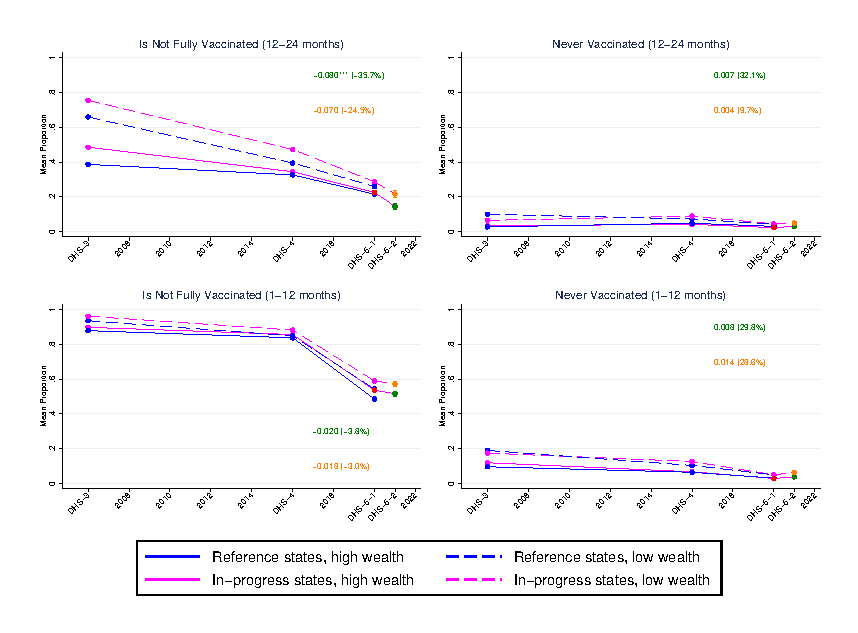
\includegraphics[width=1\linewidth]{images/meanGraphs1.eps}
\caption{\label{fig:meanGraphs1} Historical trends using previous DHS surveys in India in 2005-6 (DHS-3) and 2015-16 (DHS-4), compared to the most recent round from 2029-21 (DHS-5-1 and -2) for vaccination-specific health outcomes. Marginal effects between DHS-5-1 and DHS-5-2 are same as the main results of this thesis with preferred specification (fourth column of \cref{tab:tableLongProbit}): red, green, and orange dots representing baseline, $After$ and $After\text{ x }LowWealth$-interaction, respectively.}
\end{figure}

\begin{figure}
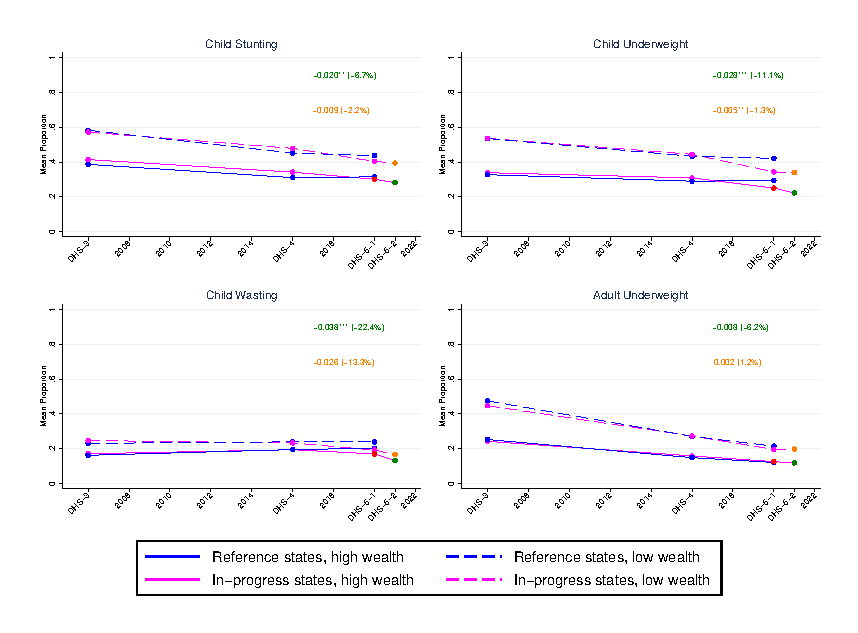
\includegraphics[width=1\linewidth]{images/meanGraphs2.eps}
\caption{\label{fig:meanGraphs2} Historical trends using previous DHS surveys in India in 2005-6 (DHS-3) and 2015-16 (DHS-4), compared to the most recent round from 2029-21 (DHS-5-1 and -2) for nutrition-specific health outcomes. Marginal effects between DHS-5-1 and DHS-5-2 are same as the main results of this thesis with preferred specification (fourth column of \cref{tab:tableLongProbit2}): red, green, and orange dots representing baseline, $After$ and $After\text{ x }LowWealth$-interaction, respectively.}
\end{figure}

\begin{figure}
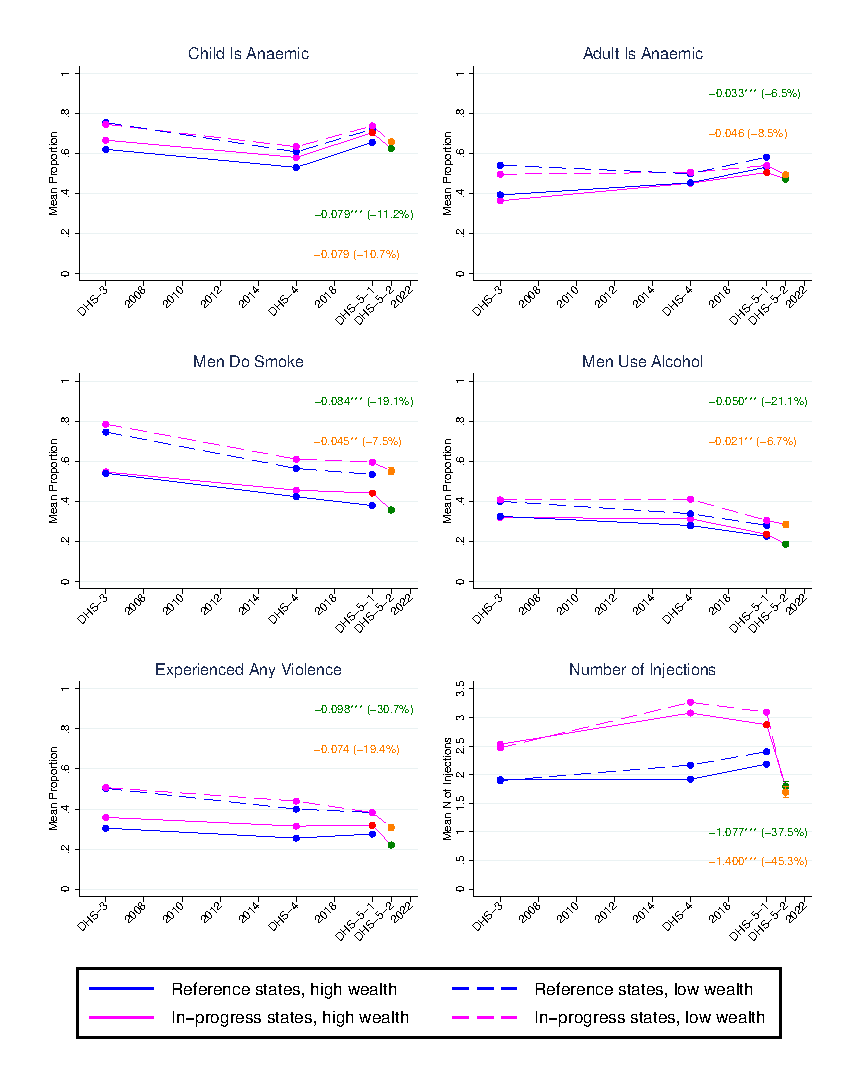
\includegraphics[width=1\linewidth]{images/meanGraphs3.eps}
\caption{\label{fig:meanGraphs3} Historical trends for other used outcomes. Please refer \cref{fig:meanGraphs1,fig:meanGraphs2} for used notation.}
\end{figure}

The result of such an analysis is presented in \cref{fig:meanGraphs1,fig:meanGraphs2,fig:meanGraphs3}. DHS-3, 4 and 5 refer to the corresponding DHS survey rounds. Mean values are calculated separately for \textit{reference-} and \textit{in-progress} states (blue and magenta, respectively), and in both categories, separately for low-wealth and high-wealth interviewees (solid and dashed line, respectively). From DHS-5-1 to DHS-5-2, the marginal effects, and standard errors for \textit{in-progress} states -- i.e., fourth column of \cref{tab:tableLongProbit,tab:tableLongProbit2,tab:tableLongProbit3,tab:tableLongProbit4} --,  are then visualized for both wealth groups. Corresponding numbers are also shown next to the marginal effect visualizations.

Along with the main result, the figures show a few important and interesting findings. First, regarding to vaccinations, left side of \cref{fig:meanGraphs1} supports the main results and such interpretation of it that something has happened in the figure development: for children aged 12-24 months, who mostly were not affected by anything related to COVID-19, the figures are following the past trend, whereas for children aged 1-12 months, mostly vulnerable for any potential effect, the trend has stopped. Second, as shown in upper right of \cref{fig:meanGraphs2}, the change in proportion of underweight children seems to approximately follow the historical trend for high-wealth interviewees, whereas the downward trend has stopped for after-lockdown low-wealth interviewees. Third -- as further discussed in \cref{subsec:discussionNutrition} --, the past worsening trend of anaemia figures from DHS-4 to DHS-5 can be clearly seen in the upper graphs of \cref{fig:meanGraphs3}, as can the subsequent significant decrease, which has occurred \textit{after-lockdowns}. Fourth, the proportion of men smoking and using alcohol, shown in middle graphs of \cref{fig:meanGraphs3}, seem to have been either following (alcohol) or clearly exceeding (smoking) the past downward trend, with extra boost most probably explained by the sale bans. And fifth, the proportion of women experiencing any violence seem to have been decreasing significantly more than the past trend, as shown in bottom-left graph of \cref{fig:meanGraphs3}.

\subsubsection{Yearly trends} \label{subsubsec:yearlyTrends}

On top of potential on-going long-term trends, a separate threat in the used model is that the measured changes may have been caused by either a regular periodical or a single but exceptional annual change, irrespective to COVID-19 pandemic. One of such yearly change might be, for example, air quality, which is heavily dependent on season and agricultural cycle -- the rice crop residues are typically burned in November and early December in India, which typically has a large impact on air pollution, and thus on certain health outcomes as well (\citet{McDonald:2020}). Another example would be the second wave of COVID-19 pandemic, a.k.a. the Delta-variant, which was exceptionally devastating in India (\citet{Salvatore:2022}).

These threats cannot be fully addressed with the data used in this thesis. State-wise data collection from previous surveys took less than a year, which means that within a single state, there is no reference data to be used for consecutive years. However, to partially address both issues, \textit{before-} and \textit{after-lockdown} data were restricted to the same time windows of January 7 to March 22, 2020, and 2021, as shown in \cref{fig:dhsHistogram}, when calculating the main results in \cref{tab:tableLongProbit,tab:tableLongProbit2,tab:tableLongProbit3,tab:tableLongProbit4}. Thus, if an unobserved cause occurred at the same time every year, this cause affected both \textit{before-} and \textit{after-lockdown} data. In addition, the Delta-variant of COVID-19 started to affect large-scale at the end of March-beginning of April 2021 (\citet{Salvatore:2022}), both directly through infection and in-directly by consequent actions. With the time windows used, Delta-variant does not affect the results either.

\subsubsection{Robustness - limit on boundaries} \label{subsubsec:limitOnBoundaries}

\begin{figure}
\begin{subfigure}{.49\textwidth}
\centering
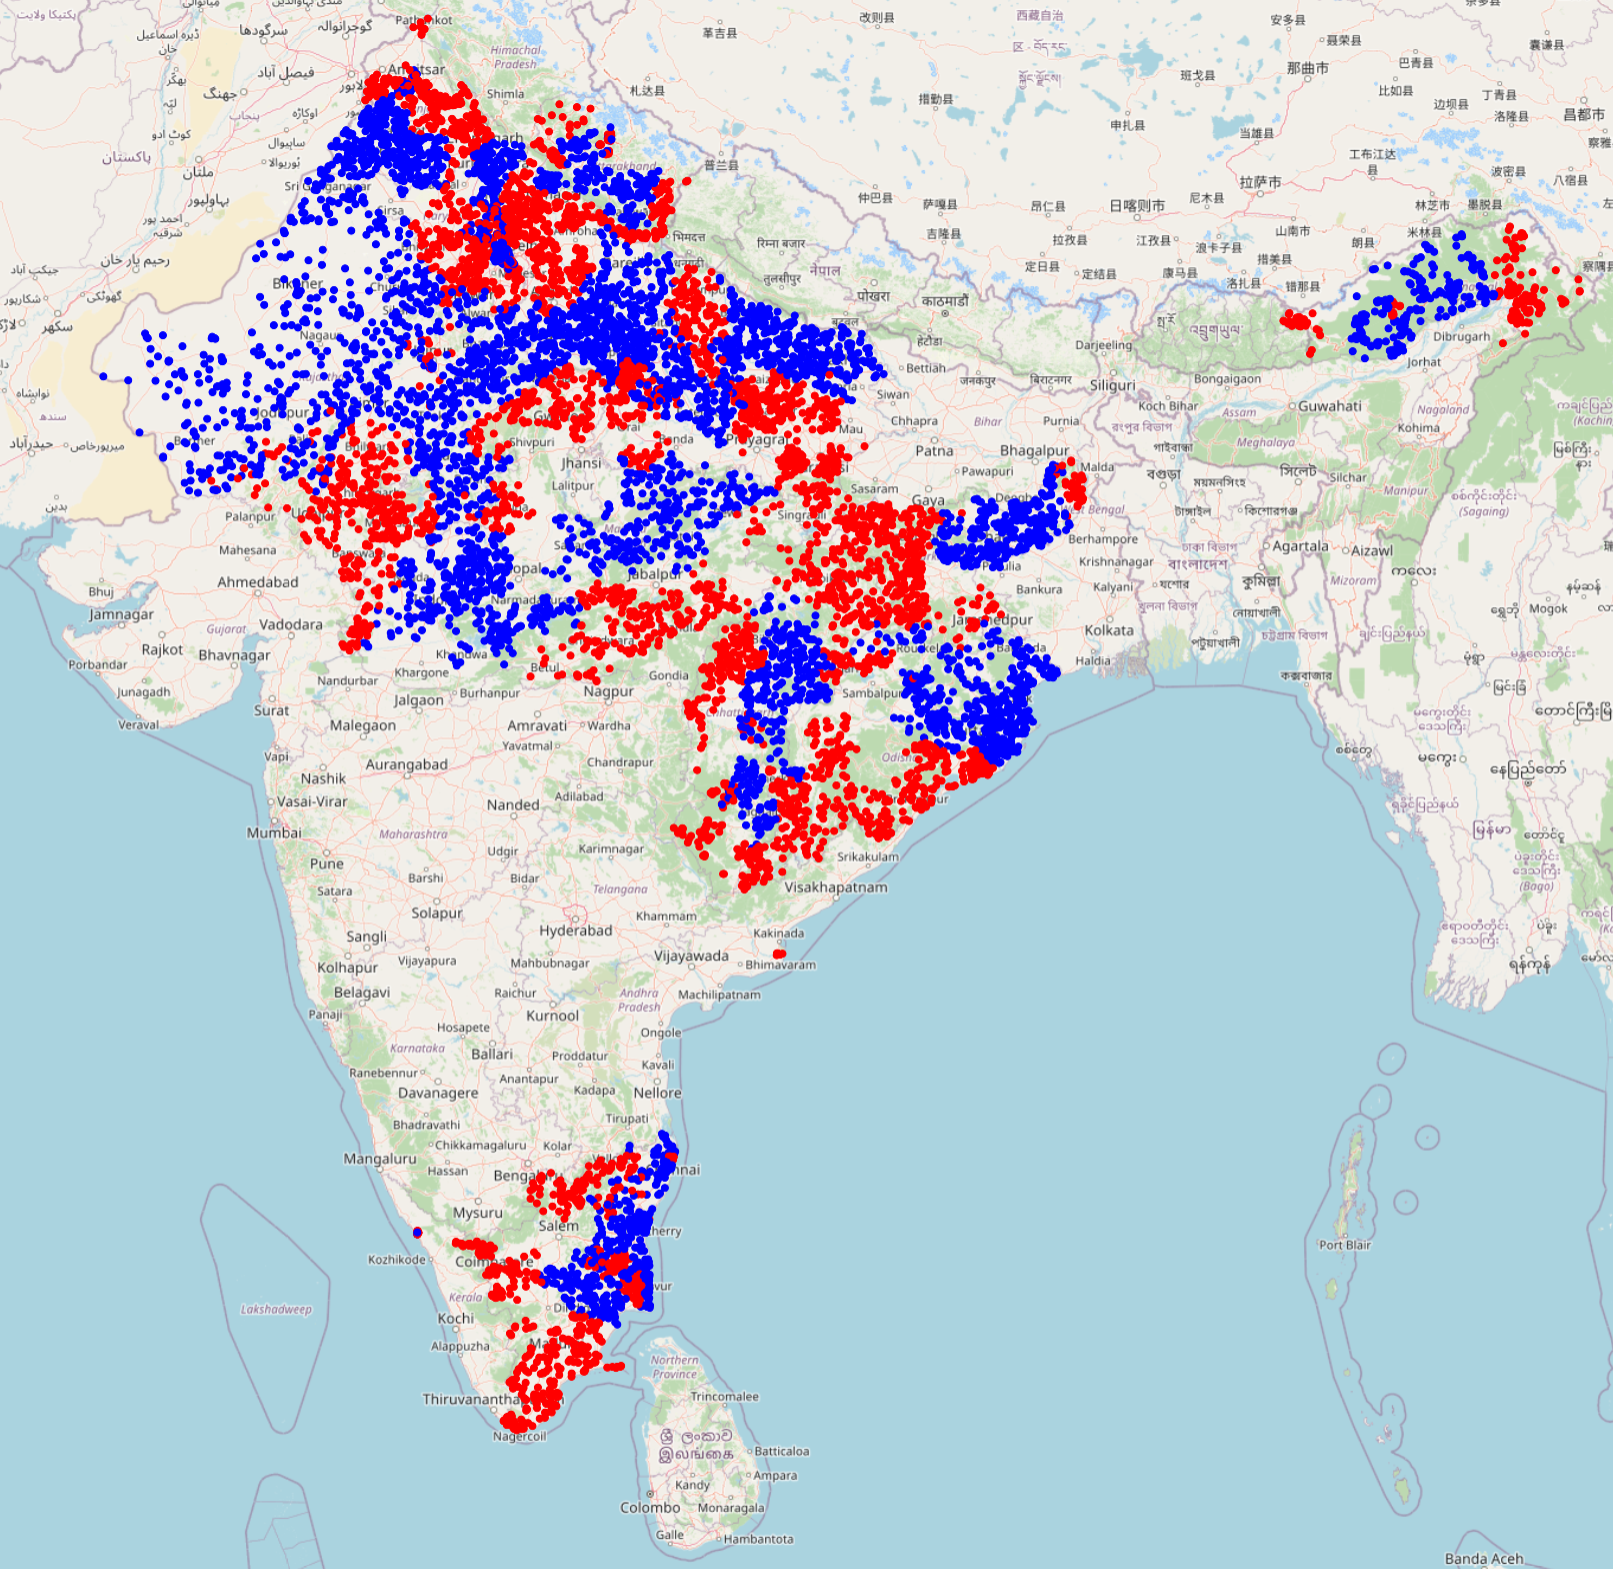
\includegraphics[width=\linewidth]{images/allDataWinterMonths.png}
\caption{ \label{fig:areas_present}}
\end{subfigure}
\begin{subfigure}{.49\textwidth}
\centering
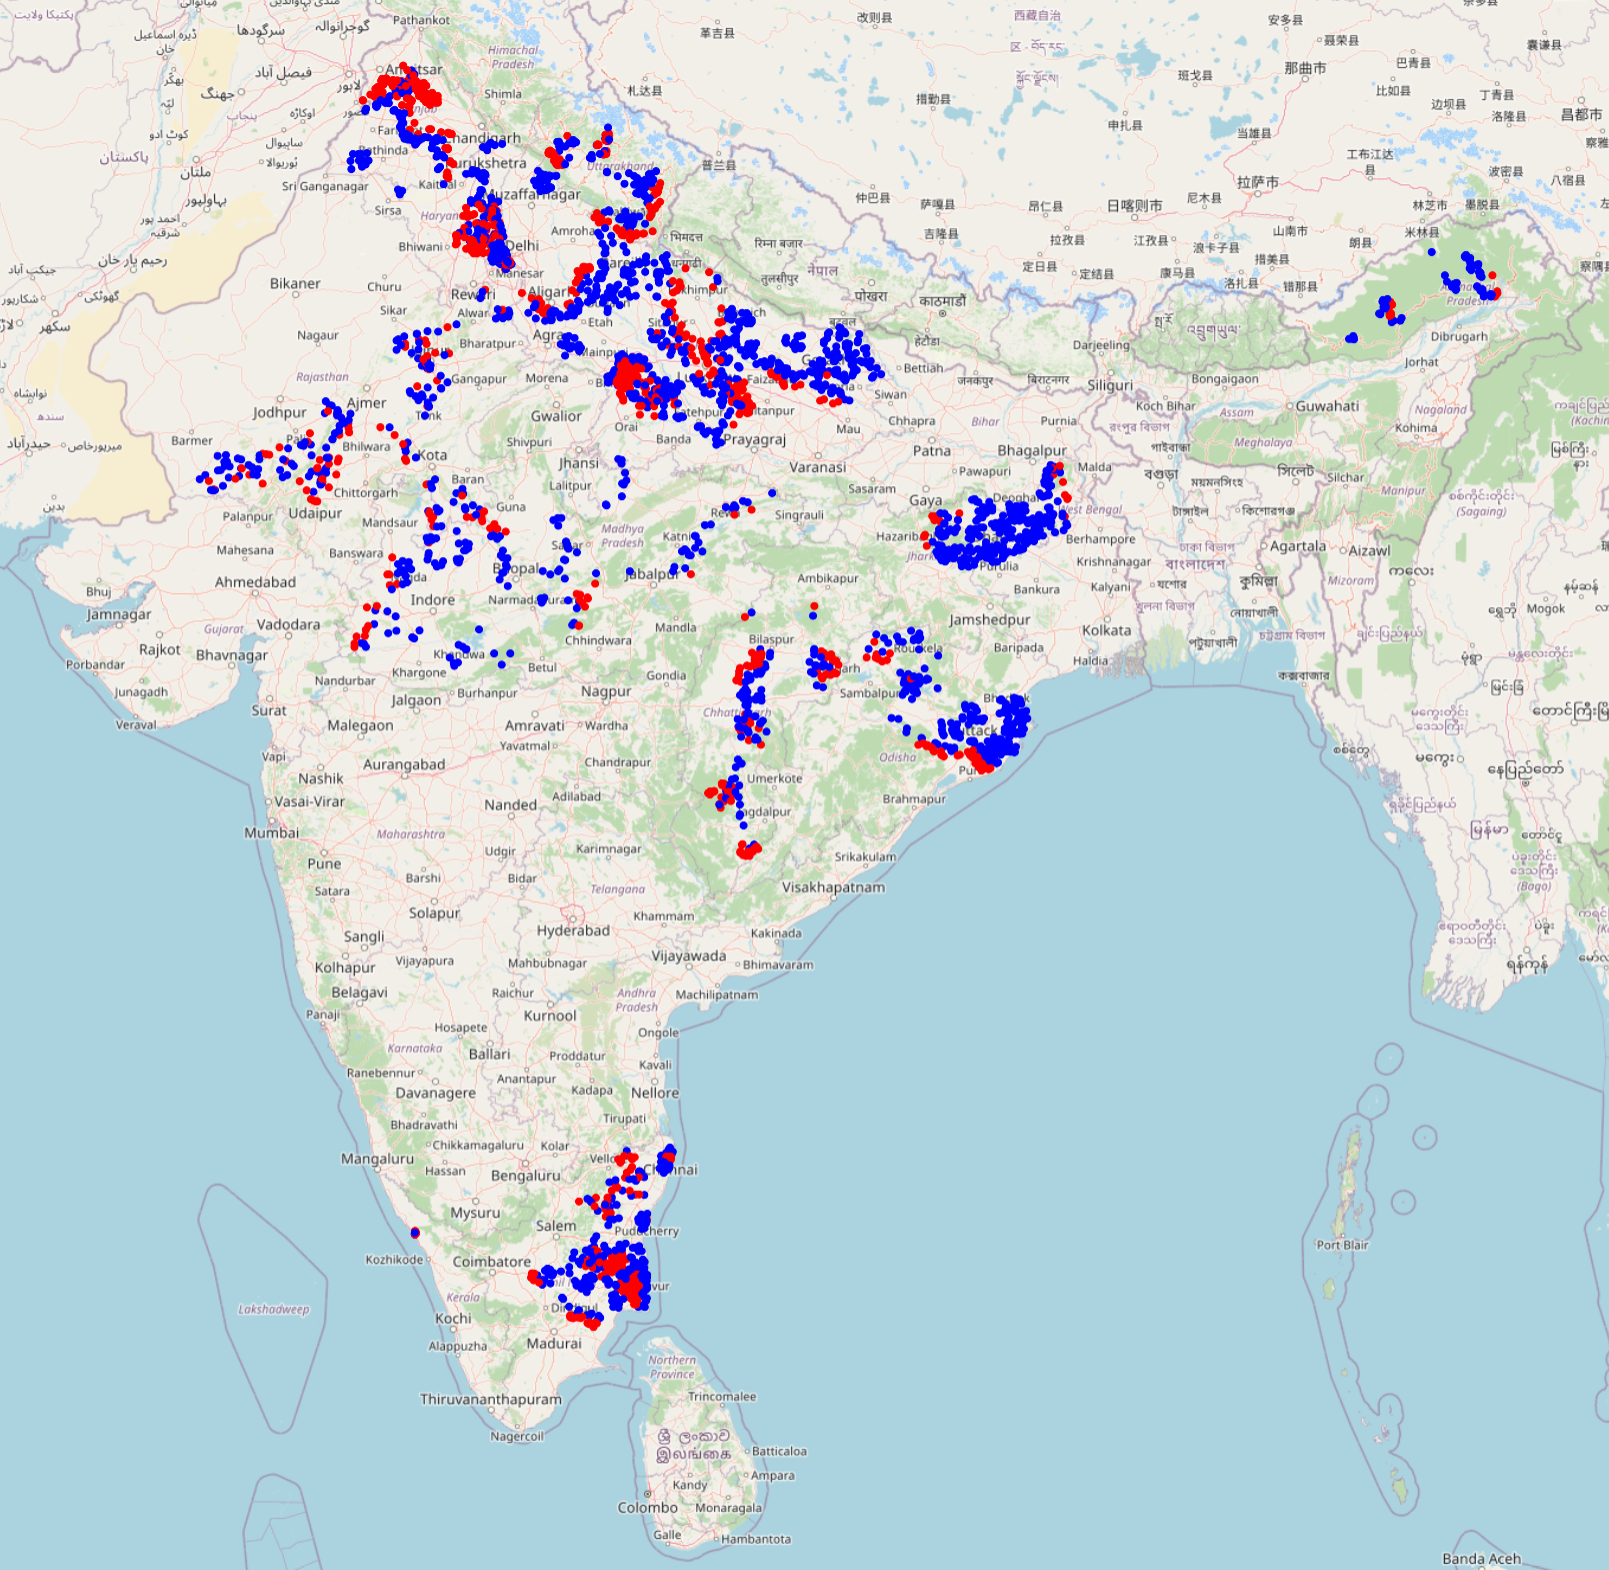
\includegraphics[width=\linewidth]{images/intraStateWinterMonths.png}
\caption{ \label{fig:areas_report}}
\end{subfigure}
\caption{\label{fig:areas} (a) All GPS-clusters from all observations that are used in main analysis in \textit{in-progress} states. Red and blue dots denote \textit{before-} and \textit{after-lockdown} observations, respectively. (b) Intra-state observations on before-after-boundaries, using boundary width of $d=20km$. In both images, \href{https://www.openstreetmap.org/copyright}{OpenStreetMap} is used as a background map.}
\end{figure}

On top of state- and region-wise (urban/rural) differences, there may be other spatial unobservables that may be associated with health outcomes. To reduce the effect of such unobservables, and to address potential threat of pre-determined data collection order potentially dependent on some unknown factor that would itself be dependent on health outcome, GPS data was utilized to limit the analysis to intra-state\textit{ before-} and \textit{after-lockdown} edges only.

More specifically, to  limit the collected observations, the following algorithm was run. For each sample, the distance along the great-circle to all neighbouring samples was calculated, and the observation was accepted only if there were any neighbouring within-state samples that were less than $d$ kilometers away ($d=20$). Thus, the analysis was restricted to intra-state \textit{before-} and \textit{after-lockdown} boundaries only, and the potential effect was calculated across these boundaries. Excluding inter-state neighbouring samples excludes the effects of state-wise differences. The data is visualized in \cref{fig:areas_present}, where in (a), all GPS clusters of the observations used in the main analysis is visualized as red and blue for \textit{before-} and \textit{after-lockdown} observations, respectively, and in (b) only the data at intra-state \textit{before-} and \textit{after-lockdown} boundaries, at a distance $d=20km$.

The results are shown in column (5) of \cref{tab:tableLongProbit,tab:tableLongProbit2,tab:tableLongProbit3,tab:tableLongProbit4}. The magnitude of the coefficient of interest is preserved for all other health outcome variables except \textit{Men Do Smoke}, but it is not statistically significant anymore for \textit{Never Vaccinated}, \textit{Child Underweight}, \textit{Men Use Alcohol} and \textit{Men Do Smoke}. However, it should be noted that the number of observations for these variables is small, which likely explains these exceptions. Therefore, it can be concluded that these figures give confidence to rely on the main analysis of this thesis.

\newpage
\section{Stringency analysis} \label{sec:stringency}

India is a very large country both in terms of area and population. Therefore, there are several factors that can cause variation in indirect pandemic effects. Presumably one of the big factors is the intensity and stringency of which government and local administration are reacting to the progress of the pandemic. This thesis explores the effect of stringency using Stringency data from Oxford COVID-19 Government Response Tracker (\citet{Hale2021}).

\subsection{Data} \label{subsec:stringencyData}

Oxford COVID-19 Government Response Tracker (OxCGRT) is a dataset that systematically collected, continuously and with comparable indices, the data on how the governments of more than 180 countries and numerous countries' sub-jurisdictions implemented policies to respond to the COVID-19 pandemic. The dataset contains comparable data on five different types of policy indicators: containment and closure policies (e.g., movement restrictions, school closures), economic policies, health system policies related to COVID-19, vaccination policies and other policies that do not fit into the previous four types. Data collection started on January 1, 2020, and data was continuously collected until the end of 2022. For India, daily data is available at the state level.

This thesis focuses on the possible indirect effects of COVID-19. Thus, OxCGRT Stringency data is used in analysis. Stringency index, for which the data was collected daily for each state, is defined as

\begin{equation} \label{eq:stringency}
    Stringency = \frac{1}{9} \sum_{j=1}^9 I_j,
\end{equation}
%
where $I_j$ is an indicator with a value from 0 to 100 pertaining to the individual policy. Each policy is flagged according to how it is applied -- locally, in specific areas/circumstances, or nationwide. When constructing the indicator value, these flags are considered so that each indicator has an equal contribution to the total index\footnote{\url{https://github.com/OxCGRT/covid-policy-tracker/blob/master/documentation/index_methodology.md} (accessed on 2023-5-7) shows the details for stringency index calculations. Reader may also refer to \citet{Hale2021}.}. The indicators $I_j$ used to calculate $Stringency$ in \cref{eq:stringency} are:
\begin{itemize}
    \item Closings of schools and universities
    \item Closings of workplaces
    \item Cancelling public events
    \item Limits on gatherings
    \item Closing of public transport
    \item Orders to "shelter-in-place" and otherwise confine to the home
    \item Restrictions on internal movement between cities/regions
    \item Restrictions on international travel
    \item Presence of public info campaigns
\end{itemize}

\begin{figure}
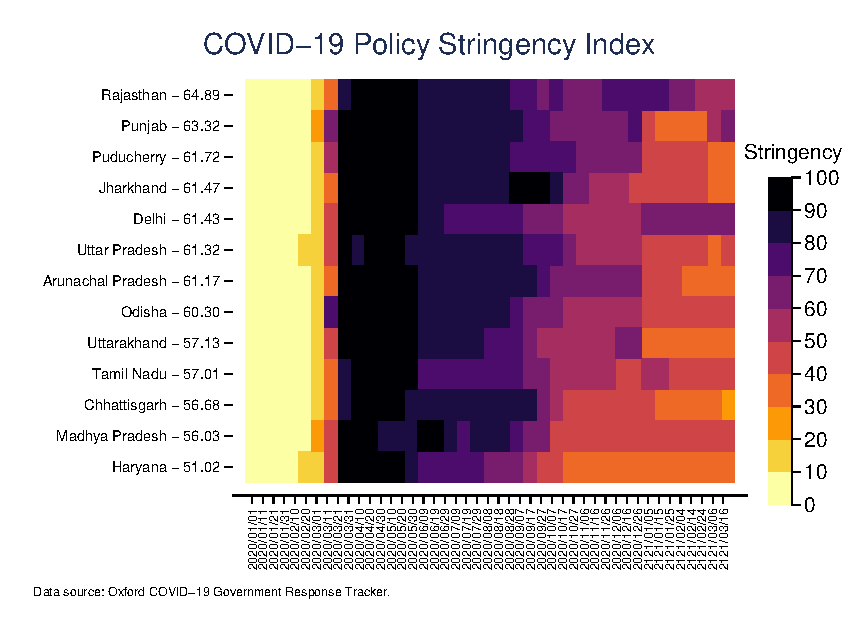
\includegraphics[width=1\linewidth]{images/stringencyIndex.eps}
\caption{\label{fig:stringency} Stringency index (\textit{Stringency} of \cref{eq:stringency}), visualized in ten-day periods between January 1, 2020, and March 20, 2021. Each line shows \textit{Stringency} for the corresponding \textit{in-progress} state included in the main analysis. The number following each state -- e.g., 64.89 for Rajasthan -- shows the daily average stringency calculated over the shown period.}
\end{figure}

Stringency indices, visualized for ten-day periods from January 1, 2020, to March 20, 2021, calculated state-wise for all \textit{in-progress} states included in the main analysis, are shown in \cref{fig:stringency}. The number after the state shows the average stringency calculated over the whole shown period. As can be seen from the visualization and from the numbers, there are no big differences between the states in terms of \textit{Stringency}.

\subsection{Model} \label{subsec:stringencyModel}

To investigate the possible effect, the stringency variable, $HiStr$, is introduced in the main models (\cref{eq:continuousModel,eq:probitModel}). As an example, the probit model (\cref{eq:probitModel}) is therefore

\begin{equation} \label{eq:stringencyProbitModel}
\begin{split}
    Pr(Y_{ijk}^h = 1) = &\Phi(\alpha^h + \beta_{1}^h After_i + \beta_{2}^h After_i \times LowWealth_i + \beta_{3}^h After_i \times HiStr_i +\\
    & + \beta_{4}^h After_i \times LowWealth_i \times HiStr_i + \gamma_1^h LowWealth_i + \\
    & \gamma_2^h HiStr_i + \gamma_3^h LowWealth_i \times HiStr_i + \delta^h X_i + State_j^h + Month_k^h),
\end{split}
\end{equation}
%
where $\beta_1$, $\beta_2$, $\beta_3$ and $\beta_4$ are the variables of interests. In terms of used controls, these models are similar to the main models. $HiStr$ is a dummy variable that takes the value 1 if the location where an individual lives, belongs to the higher 30\% when measured in terms of $Stringency$, calculated for all states included in the analysis. The states that are included in $HiStr$ are thus Rajasthan, Punjab, Puducherry, Jharkhand, and Delhi.

\subsection{Results} \label{subsec:stringencyResults}

Stringency analysis results are shown in \cref{tab:analysisStringency} for all main outcomes and using same controls as for the main analysis, showing all four estimates of interests introduced in \cref{eq:stringencyProbitModel}.

The results reveal a few interesting points in terms of further understanding the observations from the results of main analysis of this thesis. First, in terms of child underweight, when stringent region information is added into the model, \textit{after-lockdown} effect remains the same, but additionally, if a child is from most stringent areas, she is expected to be 12.8\% (-2.7+2.2+3.7=3.2\%-point) more likely to be underweight, compared to if a child is interviewed \textit{before-lockdown}. Furthermore, the child is also 6.6\% (-2.2+4.2=2.0\%-point) more likely to suffer from stunting, all these changes being statistically significant. Second, results for child and adult anaemia suggests that the significant improvement in the anaemia figures is largely reversed if an interviewee, either child or adult, is from high stringency area -- -9.6+8.9=-0.7\%-point and -4.1 + 3.0 = -1.1\%-point change anymore for child and adult, respectively. And third, consistent results with main analysis in terms of smoking among men are also observed from the stringency analysis: if interviewed \textit{after-lockdowns} in high stringency areas, men are 15.2\% (5.1\%-point) less likely smoking, as compared to lower stringency areas, and altogether 26.8\% (-6.7 - 5.1 = 11.8\%-point). This is plausible, as most presumably sales bans have made smoking simply the more difficult the stricter policies have been practiced.

\begin{table}[htbp]\centering \footnotesize \def\sym#1{\ifmmode^{#1}\else\(^{#1}\)\fi}\caption{\label{tab:analysisStringency} \footnotesize Marginal probit estimates (\cref{eq:stringencyProbitModel}) for stringency analysis}\begin{tabular}{l*{7}{c}} \hline\hline
&\rot{Not Fully Vacc, 12-24}&\rot{Never Vacc, 12-24}&\rot{Not Fully Vacc, 1-12}&\rot{Never Vacc, 1-12}&\rot{Child Stunting}&\rot{Child Underweight}&\rot{Child Wasting}\\
\textit{After}      &      -0.073\sym{***}&       0.014\sym{**} &      -0.017         &       0.011         &      -0.022\sym{**} &      -0.027\sym{***}&      -0.039\sym{***}\\
                    &     (0.018)         &     (0.006)         &     (0.016)         &     (0.008)         &     (0.011)         &     (0.009)         &     (0.009)         \\
[1em]
\textit{After} x \textit{LowWealth}&       0.010         &      -0.010         &      -0.003         &       0.004         &       0.012         &       0.022\sym{*}  &       0.016         \\
                    &     (0.023)         &     (0.008)         &     (0.020)         &     (0.009)         &     (0.012)         &     (0.012)         &     (0.011)         \\
[1em]
\textit{After} x \textit{HiStr}&      -0.002         &      -0.016         &      -0.016         &       0.002         &       0.042\sym{**} &       0.037\sym{**} &       0.018         \\
                    &     (0.027)         &     (0.012)         &     (0.028)         &     (0.013)         &     (0.020)         &     (0.017)         &     (0.017)         \\
[1em]
\textit{After} x \textit{LowWealth} x \textit{HiStr}&      -0.024         &       0.017         &       0.020         &      -0.008         &      -0.032         &      -0.028         &      -0.022         \\
                    &     (0.039)         &     (0.017)         &     (0.038)         &     (0.016)         &     (0.024)         &     (0.023)         &     (0.019)         \\
&\rot{Adult Underweight}&\rot{Child Anaemic}&\rot{Adult Anaemic}&\rot{Men Smoke}&\rot{Men Alcohol}&\rot{Exp Violence}&\rot{Number of Inj}\\
\textit{After}      &      -0.002         &      -0.096\sym{***}&      -0.041\sym{***}&      -0.067\sym{***}&      -0.042\sym{***}&      -0.101\sym{***}&      -1.143\sym{***}\\
                    &     (0.006)         &     (0.012)         &     (0.010)         &     (0.016)         &     (0.013)         &     (0.014)         &     (0.097)         \\
[1em]
\textit{After} x \textit{LowWealth}&       0.013         &       0.004         &      -0.007         &       0.026         &       0.025         &       0.015         &      -0.286\sym{**} \\
                    &     (0.008)         &     (0.012)         &     (0.011)         &     (0.019)         &     (0.015)         &     (0.019)         &     (0.121)         \\
[1em]
\textit{After} x \textit{HiStr}&      -0.021\sym{**} &       0.089\sym{***}&       0.030         &      -0.051\sym{*}  &      -0.042         &       0.022         &       0.213         \\
                    &     (0.008)         &     (0.022)         &     (0.021)         &     (0.027)         &     (0.027)         &     (0.027)         &     (0.184)         \\
[1em]
\textit{After} x \textit{LowWealth} x \textit{HiStr}&      -0.015         &       0.000         &      -0.004         &       0.040         &       0.037         &       0.037         &      -0.094         \\
                    &     (0.012)         &     (0.021)         &     (0.015)         &     (0.040)         &     (0.028)         &     (0.034)         &     (0.172)         \\
\hline\hline \multicolumn{8}{l}{\footnotesize Standard errors in parentheses}\\ \multicolumn{8}{l}{\footnotesize \sym{*} \(p<0.1\), \sym{**} \(p<0.05\), \sym{***} \(p<0.01\)}\\ \end{tabular} \\ \caption*{\textbf{After} is \textit{after-lockdown}-indicator, \textbf{LowWealth} denotes belonging to two lowest wealth quintiles, \textbf{HiStr} denotes belonging to states with higher COVID-19 stringency index, and \textbf{x} denotes interaction between dependent variables. Models are controlled for wealth status, region (urban/rural), state and month fixed effects, children age and children month of birth.} \end{table}


\newpage
\section{Discussion} \label{sec:discussion}

\subsection{Vaccination} \label{subsec:discussionVaccination}

In terms of potential long-term effects on economic outcomes, vaccination- and nutrition-related health outcomes are probably the most important ones. Like shown in \cref{subsec:resultsVaccination}, there seems to be a clear difference in the effect as compared to children aged 1-12 months, who have theoretically been affected by measures related to COVID-19. This can be observed as well when comparing the differences in long-term trends for the corresponding vaccination outcome between children aged 12-24 and 1-12 months (\cref{fig:meanGraphs1}, left side): the long-standing downward trend for children aged 12-24 has continued with the spread of COVID-19 while the decline has stopped with children aged 1-12 months.

Very recently, the literature has shown that the COVID-19-pandemic was most probably to decrease immunization coverage in India: using a mother fixed-effects regression model, \citet{Summan:2023} showed that, while the immunization coverage was vaccination-type specific, it was for some vaccinations as much as 10\% lower for after "COVID-19-affected" children. This thesis shows a similar result in a sense that there indeed seems to be differences between vaccination types. Furthermore, when compared the change and the trend between children aged 1-12 and 12-24 months, it appeared that the trend behaves better for the latter, who were less likely to be affected by COVID-19-induced (indirect) effects. It is worth noting though that the results, although being somewhat similar, are not fully identical with \citet{Summan:2023}. Even if a halt in this improving trend was detected, no corresponding, relatively large quantitative changes were measured than \citet{Summan:2023}.

\subsection{Nutrition} \label{subsec:discussionNutrition}

As shown in \cref{subsec:resultsNutrition}, nutrition-specific outcomes show no deterioration for adults, but for children the results show indications of the situation being a bit different. For high-wealth individuals, the historical trend, as shown in \cref{fig:meanGraphs2}, seems to have been decreasing, but the downward trend has stopped for \textit{after-lockdown} low-wealth interviewees. Both stringency analysis and -- especially -- detailed child-specific nutrition analysis supports the interpretation that something has happened, as for the latter one, all the nutrition indicators, MDD, MAD and MMF, were deteriorated for breastfed children. This is a finding that requires further investigation.

On the other hand, anaemia-specific health outcomes were significantly improved. This is a bit surprising, but also an interesting result. As can be seen also from \cref{fig:meanGraphs3}, the prevalence of both anaemic children and adults has been increasing since DHS-4 (\citet{Rai:2023}). The reason for this past deterioration is somewhat surprising, as the Republic of India has especially tried to intervene in the matter in recent years. According to \citet{Rai:2023}, the main reason is that the politics and interventions have been at least partially wrong, and they recommended change for means that government used. However, even if \textit{after-lockdown} DHS-5-findings are included in the figures reported by \citet{Rai:2023}, they do not tell us anything about the sharp change that appears to have occurred \textit{after-lockdown}, visualized in \cref{fig:meanGraphs3} as well.  The stringency analysis further suggests that this effect is largely reversed if an interviewee, either child or adult, is from high stringency area (\cref{tab:analysisStringency}).

As \citet{Rai:2023} points out, due to the haemoglobin measurement system used in DHS surveys, the measured haemoglobin level may be slightly higher than actual levels. However, no changes, either in the measurement system, or in equipment, have been reported between DHS-3 and DHS-5. This result needs to be investigated in more detail. Is the improvement real, and if yes, what would be the exact reason behind it? Alternatively, could there be, for example, some COVID-19-specific change in the behavior of the interviewees that could have systematically affected the measurement event? So far, this has not yet been reported in the literature.

\subsection{Other outcomes} \label{subsec:discussionOtherOutcomes}

The results concerning both alcohol and smoking levels among men seem to have improved significantly, and clearly exceeding past trends from previous DHS surveys (\cref{fig:meanGraphs3}. Presumably the main factors behind these figures are given restrictions on sales: Indian Ministry of Home Affairs (MHA) strictly banned\footnote{\href{https://www.mha.gov.in/sites/default/files/MHA\%20order\%20dt\%2015.04.2020\%2C\%20with\%20Revised\%20Consolidated\%20Guidelines\_compressed\%20\%283\%29.pdf}{Government of India, Ministry of Home Affairs, Order No. 40-3/2020-DM-I(A)}, accessed 2023-5-12} the sales of tobacco products during the lockdown, which presumably can be seen in these \textit{after-lockdown} figures as an increase in quitters. Since the increase is not that clear for low-wealth interviewees, it may be that the decrease in income was not such a big reason for the increase. Consistent results for male smoker are also observed from the stringency analysis, where the more stringent have the policies been, the less probable is a man smoking if interviewed after-lockdowns, as compared to before-lockdowns. Taking the already presented explanation of the overall decrease of proportion of smokers, the figures are plausible: smoking has simply been the more difficult the stricter policies have been implemented.

The same MHA order banned public sales of alcohol during the lockdown, which may also have been the reason that the proportion of men who drink alcohol has decreased, which, like smoking behavior, has decreased a lot. Although the long-term trend has also been decreasing (middle-right graph in \cref{fig:meanGraphs3}), the change seems to be stronger than the past trend. It should be noted here though that the variable used was simply a \textit{yes/no} answer to the question "Do you drink alcohol?". Thus, it is possible that the measure is not necessarily working as a good proxy for harmful alcohol abuse, but rather for general behavioral change. For example, if an interviewee who only goes to bars or other public restaurants has stopped going there since the COVID-19 lockdowns, he might answer \textit{no}, instead of the previous \textit{yes}. Like \citet{OECD:2021} shows, drinking habits have changed dramatically since the onset of COVID-19, with people perhaps consuming more alcohol at home.

The significant decrease of women experiencing domestic violence is somewhat surprising. During the lockdown, it was reported that domestic violence cases increased in India\footnote{Times of India: \href{https://timesofindia.indiatimes.com/life-style/relationships/love-sex/domestic-violence-cases-in-india-on-the-rise-during-lockdown-says-report/articleshow/75801752.cms}{"Domestic violence cases in India on the rise during lockdown, says report"}, published May 18, 2020, accessed May 12, 2023}, and this is also supported in the literature later (e.g., \citet{Sanches:2020}), although Indian-specific review does not seem to exist yet. However, \citet{Sanches:2020}, and all other figures in the literature as well, seem to cover only the first weeks of the first wave of COVID-19. Hence, it may be possible that the quick recovery from the first wave and from the corresponding lockdowns reduced domestic violence quite dramatically by the beginning of 2021. On the other hand, something may have changed in the practical arrangements by the surveyors, which may affect this specific question. An obvious explanation, the presence of other people during the survey, seems not to have increased \textit{after-lockdowns}.

Lastly, number of injections that women has received in the last 12 months seems to have decreased significantly. If this change had happened in the long run, it would have been interpreted as an improvement. In developing countries, injections are used more than in developed countries, because oral drugs are many times more expensive, and thus not necessarily available. However, the risk of using injections is high, because hygiene practices may not be at a good enough level and the syringes can therefore cause infections. For this reason, reducing the number of injections can usually be considered a goal. However, it is not likely -- especially given the past trend, shown in \cref{fig:meanGraphs3} -- that such a decrease in such a short time would have been compensated for using oral medications. A more likely explanation is that the figure serves as a proxy for the frequency of visits to the health center. Most likely, women have just visited health center less, either due to a lack of resources or due to new deficiencies in the healthcare system that have appeared since the start of the COVID-19 pandemic.

\subsection{Limitations} \label{subsec:limitations}

The main limitation of the used approach is that the time difference between \textit{before-} and \textit{after-lockdown}-observations is long. Because the data collection process was suspended for at least six months, and because the data is further limited to time windows between January and March 2020 and 2021, other types of unobservables, not necessarily related to any indirect COVID-19-induced effects, may have been associated with the used outcome variables. A model similar to \citet{Bassi:2017} is used. However, since exposure to the Papal visit, which \citet{Bassi:2017} uses as a source of persuasion, lasted only a couple of days, there is no plausible explanation for what else would have caused the measured changes in short-term beliefs, such as intentions to contraception. In this work, the gap is longer. With the help of the trends from the past DHS surveys (\cref{subsubsec:trends}), as well as other robustness checks, the probability of occasional and/or COVID-19-unrelated change acting as a root cause for the measured changes is mitigated. However, with DHS data alone, other shorter but still temporal changes, or changes in behavior as the root cause for changes cannot be fully ruled out.

\newpage
\section{Conclusion} \label{sec:conclusion}

In this thesis, it was studied whether there have been changes on health outcomes in developing countries through indirect channels during the COVID-19 pandemic. Limiting the focus to the first wave of COVID-19 and to India made it possible to isolate the effects via indirect channels from the possible effects of directly infected people. The research began by introducing the connection between health and economic development, as well as introducing the literature of how certain health outcomes are affecting later economic outcomes. This information was then used to select outcomes of interest in the empirical section, which was conducted using the data from fifth DHS survey of India. In an empirical section, a model was built to investigate possible changes that might have happened during the first wave of COVID-19 pandemic. In addition, different additional validation and robustness checks were built and run for the built model, as well as balancing tests for the used DHS data.

The results were twofold. India's good progress in improving immunization coverage over the past few years was found to have stalled among children who were potentially exposed to the influence of COVID-19-related effects. A similar downward trend seems to have stopped in terms of underweight children among low-wealth interviewees. The detailed nutritional analysis showed that the breastfed children have worse nutritional and dietary outcomes, as the probability that all children did not meet both MDD and MAD requirements, and the MMF requirements for low-income children, had increased. Chronic nutrition measures were also worse in high stringency areas. For all these changes, difference was statistically significant if interviewed \textit{after-lockdown}.

On the other hand, the recent deterioration in the proportion of anaemic people appears to have been reversed during the first year of COVID-19 pandemic, and the reduction in the proportion of anaemic children and adults was significant, being mostly driven by lower-stringency areas. In addition, all results for alcohol use, smoking and experiencing domestic violence improved significantly compared to the past trends.

These results are important both from a preventive and curative point of view. The results indicate that such sudden and full lockdowns imposed by India between March and May 2020 may have had implications on health outcomes and should be avoided. Nutritional analysis conducted among young children aged 6-24 months may require specific considerations, as the figures revealed consistent deficiency in terms of breastfed children, which may have potentially long-term effects on this generation. In addition, while no clear decrease in overall immunization coverage was observed, the improvement in the previous trend was found to have clearly stopped, which is in line with recent literature, where an overall decrease has been shown to have occurred in India as well.

There are several directions that are to be headed for future research. First, a more detailed analysis for possible explanatory variables could be considered. One option, just to mention one, would be an occupation -- as an example, it would be beneficial to investigate which types of occupations are affected most. Second, the temporal difference (\cref{subsec:limitations}) could be addressed with some other dataset and/or event, preferably one that causes exogenous variation in terms of COVID-19-start, which could then potentially be used to demonstrate the existence or non-existence of causal effect of COVID-19 on health outcome through indirect channels. Third, somewhat surprising findings, such as clear improvement in \textit{Experienced Any Violence}-figures, and possible root causes behind these figures, could be further investigated.

\newpage
\bibliography{references/report.bib}

\newpage
\begin{appendices}

\setcounter{table}{0}

\renewcommand{\thetable}{A\arabic{table}}

\setcounter{figure}{0}

\renewcommand{\thefigure}{A\arabic{figure}}

\begin{table}[htbp]\centering \tiny \caption{\label{tab:balanced} Balancing checks of used controls on vaccination-specific health outcomes}
\begin{tabular}{l*{4}{c}}
\hline\hline
            &           N&      Before&       After&P-value (Before==After)\\
\hline
Is Not Fully Vaccinated (Aged 12-24)&            &            &            &            \\
Low Wealth  &       16808&       0.448&       0.455&       0.356\\
Is Urban    &       16808&       0.209&       0.200&       0.734\\
Hindi       &       16808&       0.832&       0.812&       0.009\\
Muslim      &       16808&       0.084&       0.101&       0.094\\
Christian   &       16808&       0.026&       0.029&       0.013\\
Sikh        &       16808&       0.041&       0.027&       0.954\\
Scheduled Caste&       16633&       0.262&       0.220&       0.053\\
Scheduled Tribe&       16633&       0.120&       0.203&       0.054\\
Age in Months&       16808&      17.138&      17.249&       0.192\\
Sex         &       16808&       0.476&       0.475&       0.726\\
\hline
Never Vaccinated (12-24)&            &            &            &            \\
Low Wealth  &       16808&       0.448&       0.455&       0.356\\
Is Urban    &       16808&       0.209&       0.200&       0.734\\
Hindi       &       16808&       0.832&       0.812&       0.009\\
Muslim      &       16808&       0.084&       0.101&       0.094\\
Christian   &       16808&       0.026&       0.029&       0.013\\
Sikh        &       16808&       0.041&       0.027&       0.954\\
Scheduled Caste&       16633&       0.262&       0.220&       0.053\\
Scheduled Tribe&       16633&       0.120&       0.203&       0.054\\
Age in Months&       16808&      17.138&      17.249&       0.192\\
Sex         &       16808&       0.476&       0.475&       0.726\\
\hline
Is Not Fully Vaccinated (1-12)&            &            &            &            \\
Low Wealth  &       16260&       0.448&       0.455&       0.770\\
Is Urban    &       16260&       0.195&       0.192&       0.642\\
Hindi       &       16260&       0.837&       0.811&       0.004\\
Muslim      &       16260&       0.084&       0.102&       0.055\\
Christian   &       16260&       0.025&       0.034&       0.006\\
Sikh        &       16260&       0.038&       0.026&       0.853\\
Scheduled Caste&       16084&       0.265&       0.229&       0.301\\
Scheduled Tribe&       16084&       0.124&       0.209&       0.058\\
Age in Months&       16260&       5.610&       5.640&       0.168\\
Sex         &       16260&       0.475&       0.487&       0.727\\
\hline
Never Vaccinated (1-12)&            &            &            &            \\
Low Wealth  &       16260&       0.448&       0.455&       0.770\\
Is Urban    &       16260&       0.195&       0.192&       0.642\\
Hindi       &       16260&       0.837&       0.811&       0.004\\
Muslim      &       16260&       0.084&       0.102&       0.055\\
Christian   &       16260&       0.025&       0.034&       0.006\\
Sikh        &       16260&       0.038&       0.026&       0.853\\
Scheduled Caste&       16084&       0.265&       0.229&       0.301\\
Scheduled Tribe&       16084&       0.124&       0.209&       0.058\\
Age in Months&       16260&       5.610&       5.640&       0.168\\
Sex         &       16260&       0.475&       0.487&       0.727\\
\hline\hline
\end{tabular}

\caption*{\textbf{N} shows the used sample size. \textbf{Before} and \textbf{After} are proportions of control in question \textit{before}- and \textit{after-lockdown}, respectively. \textbf{P-value (Before == After)} shows the p-value of the corresponding equality test. OLS regression is used to perform the test of equality, in order to use DHS importance weights. }
\end{table}

\begin{table}[htbp]\centering \tiny \caption{\label{tab:balanced2} Balancing checks of used controls on nutrition-specific health outcomes}
\begin{tabular}{l*{4}{c}}
\hline\hline
            &           N&      Before&       After&P-value (Before==After)\\
\hline
Child Stunting&            &            &            &            \\
Low Wealth  &       80224&       0.463&       0.466&       0.583\\
Is Urban    &       80224&       0.208&       0.194&       0.928\\
Hindi       &       80224&       0.826&       0.815&       0.017\\
Muslim      &       80224&       0.085&       0.096&       0.147\\
Christian   &       80224&       0.029&       0.034&       0.004\\
Sikh        &       80224&       0.041&       0.026&       1.000\\
Scheduled Caste&       79388&       0.262&       0.221&       0.057\\
Scheduled Tribe&       79388&       0.124&       0.211&       0.033\\
Age in Months&       80224&      29.987&      29.366&       0.000\\
Sex         &       80224&       0.479&       0.480&       0.867\\
\hline
Child Underweight&            &            &            &            \\
Low Wealth  &       82137&       0.463&       0.467&       0.595\\
Is Urban    &       82137&       0.208&       0.195&       0.948\\
Hindi       &       82137&       0.826&       0.814&       0.016\\
Muslim      &       82137&       0.085&       0.097&       0.142\\
Christian   &       82137&       0.029&       0.033&       0.004\\
Sikh        &       82137&       0.041&       0.026&       0.978\\
Scheduled Caste&       81271&       0.262&       0.222&       0.078\\
Scheduled Tribe&       81271&       0.126&       0.211&       0.035\\
Age in Months&       82137&      29.553&      29.146&       0.000\\
Sex         &       82137&       0.479&       0.479&       0.829\\
\hline
Child Wasting&            &            &            &            \\
Low Wealth  &       79231&       0.463&       0.467&       0.635\\
Is Urban    &       79231&       0.209&       0.193&       0.865\\
Hindi       &       79231&       0.827&       0.816&       0.017\\
Muslim      &       79231&       0.084&       0.096&       0.143\\
Christian   &       79231&       0.029&       0.033&       0.005\\
Sikh        &       79231&       0.042&       0.026&       0.988\\
Scheduled Caste&       78396&       0.263&       0.222&       0.058\\
Scheduled Tribe&       78396&       0.123&       0.210&       0.029\\
Age in Months&       79231&      29.995&      29.422&       0.000\\
Sex         &       79231&       0.481&       0.479&       0.541\\
\hline
Adult Underweight&            &            &            &            \\
Low Wealth  &      259046&       0.406&       0.415&       0.773\\
Is Urban    &      259046&       0.259&       0.247&       0.885\\
Hindi       &      259046&       0.826&       0.825&       0.043\\
Muslim      &      259046&       0.064&       0.073&       0.181\\
Christian   &      259046&       0.031&       0.035&       0.010\\
Sikh        &      259046&       0.055&       0.035&       0.909\\
Scheduled Caste&      255912&       0.240&       0.214&       0.299\\
Scheduled Tribe&      255912&       0.130&       0.191&       0.119\\
Age in Years&      259046&      32.312&      32.487&       0.127\\
Sex         &      259046&       0.872&       0.868&       0.701\\
\hline\hline
\end{tabular}

\caption*{\textbf{N} shows the used sample size. \textbf{Before} and \textbf{After} are proportions of control in question \textit{before}- and \textit{after-lockdown}, respectively. \textbf{P-value (Before == After)} shows the p-value of the corresponding equality test. OLS regression is used to perform the test of equality, in order to use DHS importance weights. }
\end{table}

\begin{table}[htbp]\centering \tiny \caption{\label{tab:balanced3} Balancing checks of used controls on anemia level-, smoking usage- and alcohol usage-specific outcomes}
\begin{tabular}{l*{4}{c}}
\hline\hline
            &           N&      Before&       After&P-value (Before==After)\\
\hline
Child Is Anemic&            &            &            &            \\
Low Wealth  &       71848&       0.465&       0.469&       0.599\\
Is Urban    &       71848&       0.207&       0.195&       0.941\\
Hindi       &       71848&       0.823&       0.815&       0.036\\
Muslim      &       71848&       0.087&       0.094&       0.264\\
Christian   &       71848&       0.029&       0.035&       0.003\\
Sikh        &       71848&       0.042&       0.025&       0.893\\
Scheduled Caste&       71120&       0.269&       0.227&       0.047\\
Scheduled Tribe&       71120&       0.131&       0.218&       0.038\\
Age in Months&       71848&      33.045&      32.686&       0.001\\
Sex         &       71848&       0.478&       0.477&       0.860\\
\hline
Adult Is Anemic&            &            &            &            \\
Low Wealth  &      271700&       0.408&       0.418&       0.830\\
Is Urban    &      271700&       0.254&       0.242&       0.890\\
Hindi       &      271700&       0.825&       0.826&       0.056\\
Muslim      &      271700&       0.066&       0.073&       0.268\\
Christian   &      271700&       0.031&       0.035&       0.006\\
Sikh        &      271700&       0.054&       0.034&       0.831\\
Scheduled Caste&      268610&       0.248&       0.219&       0.168\\
Scheduled Tribe&      268610&       0.134&       0.194&       0.128\\
Age in Years&      271700&      31.879&      32.098&       0.047\\
Sex         &      271700&       0.881&       0.876&       0.271\\
\hline
Men Do Smoke&            &            &            &            \\
Low Wealth  &       34863&       0.407&       0.414&       0.630\\
Is Urban    &       34863&       0.272&       0.260&       0.643\\
Hindi       &       34863&       0.832&       0.833&       0.046\\
Muslim      &       34863&       0.060&       0.069&       0.062\\
Christian   &       34863&       0.025&       0.032&       0.019\\
Sikh        &       34863&       0.060&       0.036&       0.971\\
Scheduled Caste&       34457&       0.241&       0.220&       0.393\\
Scheduled Tribe&       34457&       0.129&       0.187&       0.131\\
Age in Years&       34863&      33.719&      33.796&       0.554\\
\hline
Men Use Alcohol&            &            &            &            \\
Low Wealth  &       34863&       0.407&       0.414&       0.630\\
Is Urban    &       34863&       0.272&       0.260&       0.643\\
Hindi       &       34863&       0.832&       0.833&       0.046\\
Muslim      &       34863&       0.060&       0.069&       0.062\\
Christian   &       34863&       0.025&       0.032&       0.019\\
Sikh        &       34863&       0.060&       0.036&       0.971\\
Scheduled Caste&       34457&       0.241&       0.220&       0.393\\
Scheduled Tribe&       34457&       0.129&       0.187&       0.131\\
Age in Years&       34863&      33.719&      33.796&       0.554\\
\hline\hline
\end{tabular}

\caption*{\textbf{N} shows the used sample size. \textbf{Before} and \textbf{After} are proportions of control in question \textit{before}- and \textit{after-lockdown}, respectively. \textbf{P-value (Before == After)} shows the p-value of the corresponding equality test. OLS regression is used to perform the test of equality, in order to use DHS importance weights. }
\end{table}

\begin{table}[htbp]\centering \tiny \caption{\label{tab:balanced4} Balancing checks of used controls on domestic violence- and number of injections-specific outcomes}
\begin{tabular}{l*{4}{c}}
\hline\hline
            &           N&      Before&       After&P-value (Before==After)\\
\hline
Experienced Any Violence&            &            &            &            \\
Low Wealth  &       23965&       0.438&       0.450&       0.940\\
Is Urban    &       23965&       0.249&       0.243&       0.649\\
Hindi       &       23965&       0.832&       0.823&       0.030\\
Muslim      &       23965&       0.065&       0.073&       0.203\\
Christian   &       23965&       0.028&       0.036&       0.018\\
Sikh        &       23965&       0.054&       0.034&       0.975\\
Scheduled Caste&       23702&       0.237&       0.212&       0.433\\
Scheduled Tribe&       23702&       0.134&       0.199&       0.160\\
Age in Years&       23965&      33.783&      33.984&       0.165\\
\hline
Number of Injections&            &            &            &            \\
Low Wealth  &      275055&       0.413&       0.419&       0.607\\
Is Urban    &      275055&       0.255&       0.246&       0.767\\
Hindi       &      275055&       0.825&       0.817&       0.024\\
Muslim      &      275055&       0.069&       0.081&       0.123\\
Christian   &      275055&       0.031&       0.034&       0.012\\
Sikh        &      275055&       0.053&       0.036&       0.999\\
Scheduled Caste&      271687&       0.241&       0.215&       0.290\\
Scheduled Tribe&      271687&       0.127&       0.189&       0.133\\
Age in Years&      275055&      29.963&      30.244&       0.049\\
\hline\hline
\end{tabular}

\caption*{\textbf{N} shows the used sample size. \textbf{Before} and \textbf{After} are proportions of control in question \textit{before}- and \textit{after-lockdown}, respectively. \textbf{P-value (Before == After)} shows the p-value of the corresponding equality test. OLS regression is used to perform the test of equality, in order to use DHS importance weights. }
\end{table}

\end{appendices}

\end{document}